\chapter{LHC-ATLAS実験}\label{chapter2}
\label{chapter2}

LHC-ATLAS実験とは、Large Hadron Collider~(LHC)\cite{article:LHC}を用いた高エネルギーの陽子–陽子衝突によって生成された粒子をATLAS~(A Troidal LHC ApparatuS)検出器によって検出し、標準模型の精密測定や新粒子探索などを行う実験である\cite{article:ATLAS}。
LHCは2018年にRun-2を終了し、2019年から2021年にかけてLHC及びATLAS検出器のアップグレード\cite{article:phase-1}が行われ、2022年からはRun-3として運転を再開している。

本章では、Run-3におけるLHC及びATLAS検出器の概要とATLA 実験で採用されているトリガーシステムについて述べる。

\section{LHC加速器}
\label{section2-1}
Large Hadron Collider~(LHC)は、スイスのジュネーブ郊外にある欧州素粒子原子核研究機構~(CERN)\cite{article:CERN}の地下に建設された周長約27km の世界最大の大型ハドロン衝突型加速器である。LHCの全体像を図\ref{fig:LHC_overview}に示す\cite{article:Overall_view_LHC}。
LHCは重心系エネルギー14TeV、瞬間ルミノシティ$1.0\times10^{34}$~cm$^{-2}$s$^{-1}$ で陽子-陽子衝突が可能なように設計されている。

\begin{figure}[tb]
  \centering
  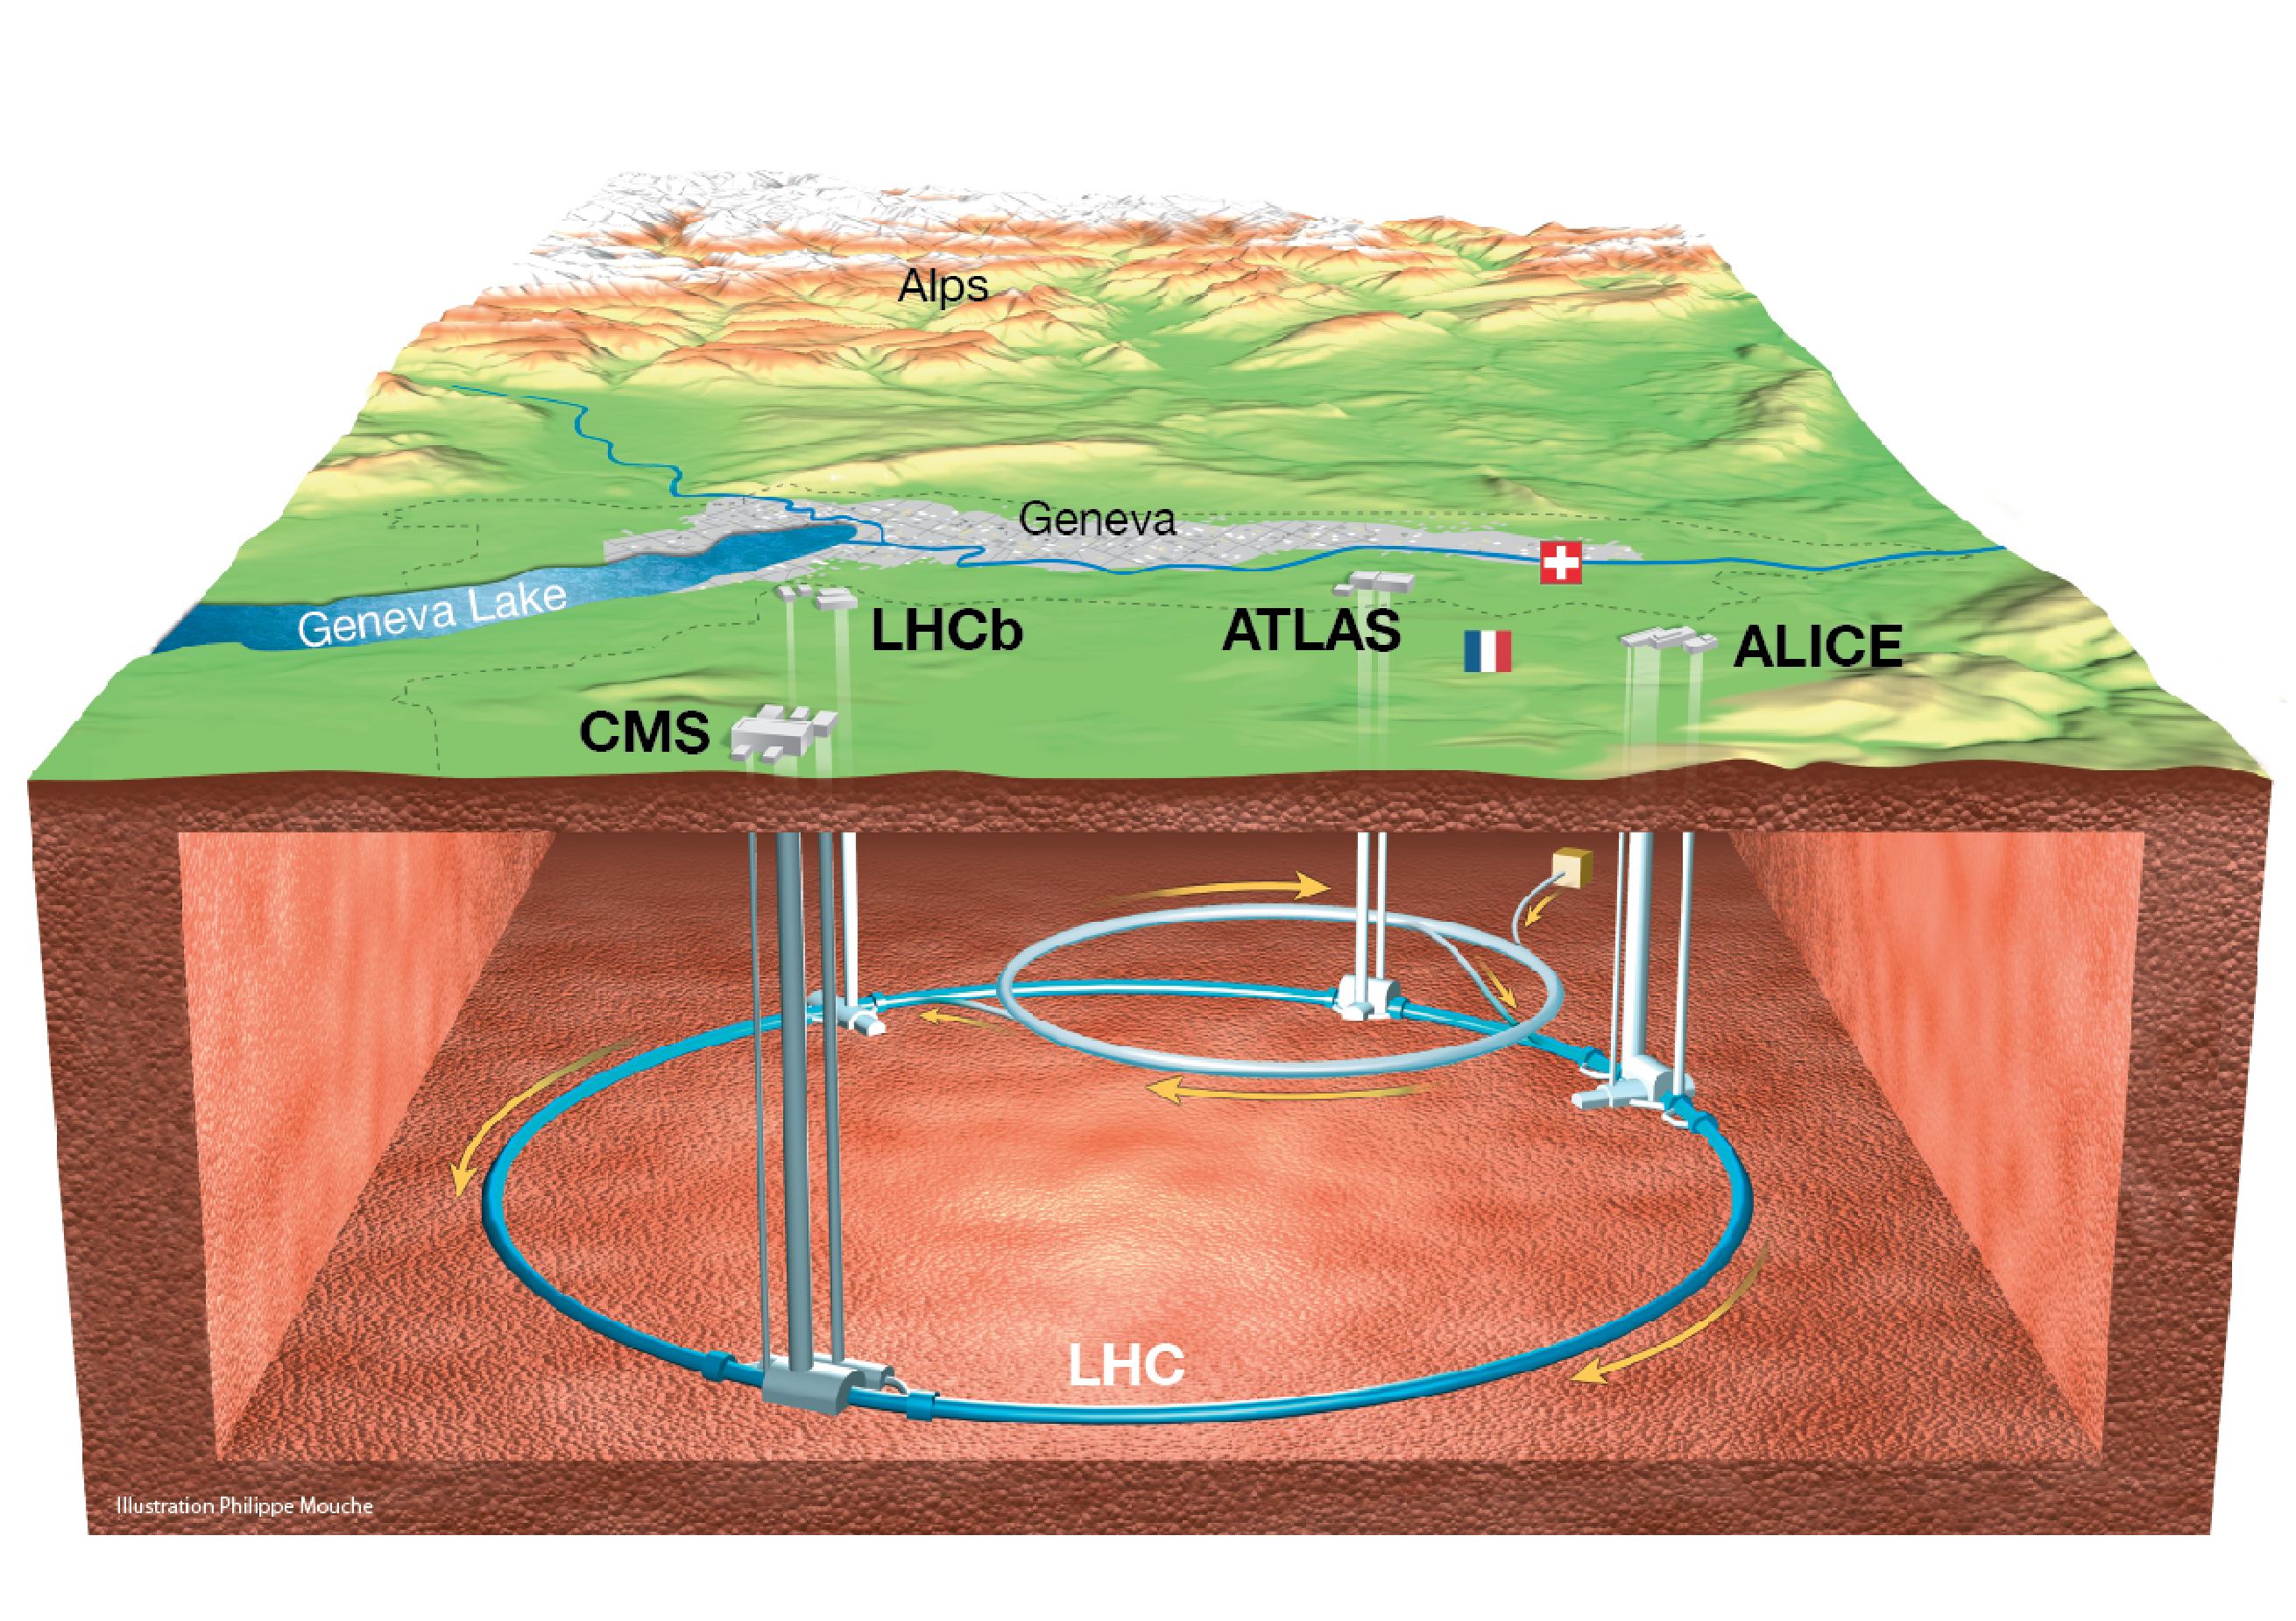
\includegraphics[clip, width=14cm]{fig/2/LHC_overview.pdf}
  \caption{LHC加速器の全体図\cite{article:Overall_view_LHC}。}
  \label{fig:LHC_overview}
\end{figure}

\begin{figure}[tb]
  \centering
  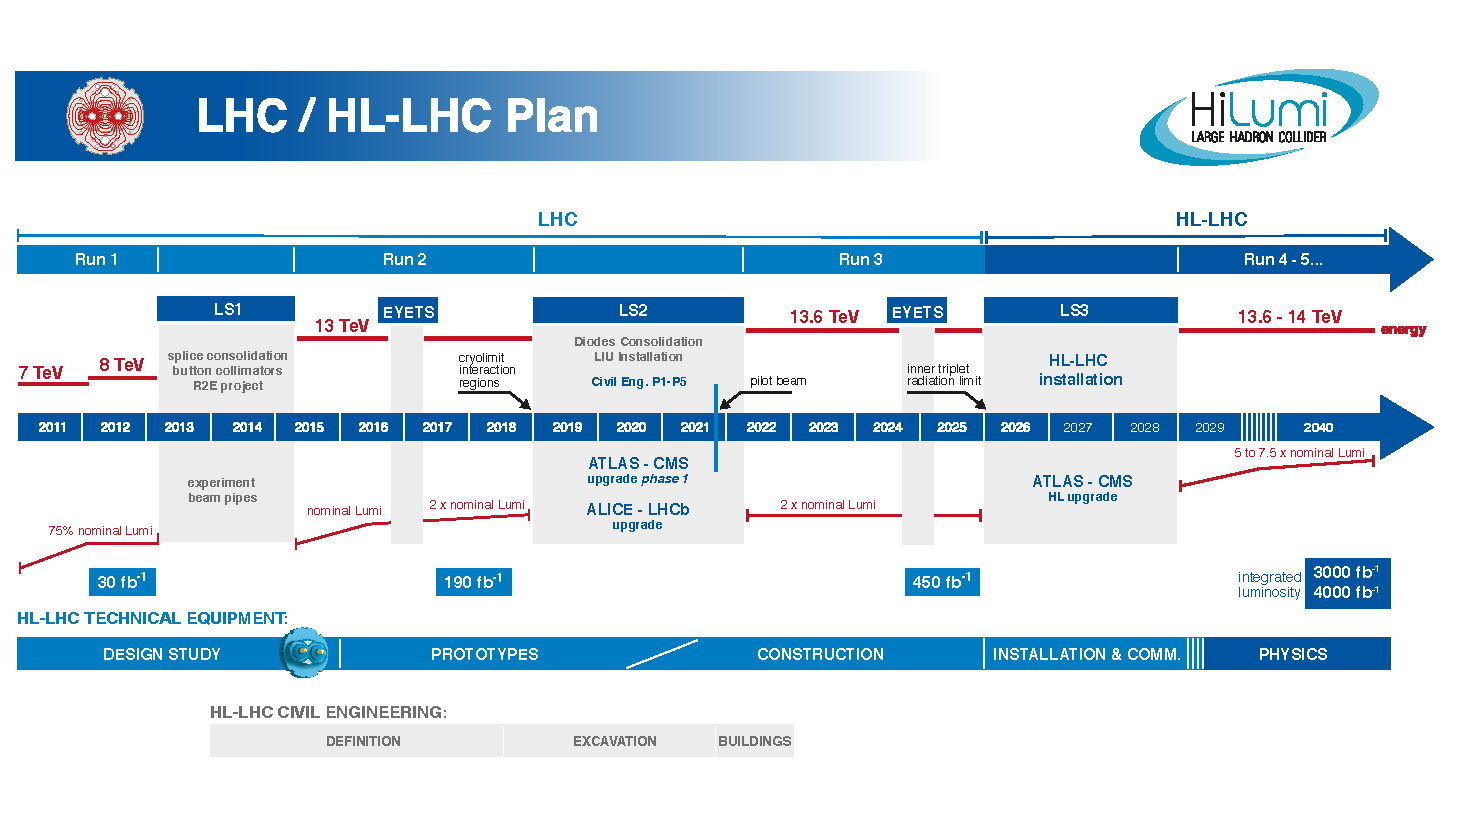
\includegraphics[clip, width=14cm]{fig/1/HL-LHC_Janvier2022.pdf}
  \caption{LHC 加速器の運転とアップグレード計画。LHC では2019年から2022年初旬までの間に Phase-1 Upgrade が行われ、現在は Run-3 として運転を再開している\cite{article:LHCDesignReport}。}
  \label{fig:LHC_Plan}
\end{figure}

LHCは2010年から本格的に実験を開始し、2010年から2012年にかけて行われた運転をRun-1、2015年から2018年にかけて行われた運転をRun-2と呼ぶ。図\ref{fig:LHC_Plan}にLHC加速器の運転計画を示す\cite{article:LHCDesignReport}。
Run-1では重心系エネルギー7-8~TeV、瞬間最高ルミノシティ$0.77\times10^{34}$~cm$^{-2}$s$^{-1}$での運転を行い、Run-2では重心系エネルギー13~TeV、瞬間最高ルミノシティ$2.0\times10^{34}$~cm$^{-2}$s$^{-1}$での運転を行った。
2019年から2021年初旬までに期間に加速器のアップグレードが行われ、2022年初旬から2025年にかけて行われるRun-3では陽子-陽子衝突の重心系エネルギーを 13.6~TeV、瞬間ルミノシティ2.0$\times$10$^{34}$~cm$^{-2}$s$^{-1}$での運転を行い、Run-2で取得したデータと合わせて積分ルミノシティ350~fb$^{-1}$のデータを取得する予定である。さらにその後、アップグレードを経て2029年からは高輝度LHC-ATLAS実験の運転が予定されている。

\begin{figure}[tb]
  \centering
  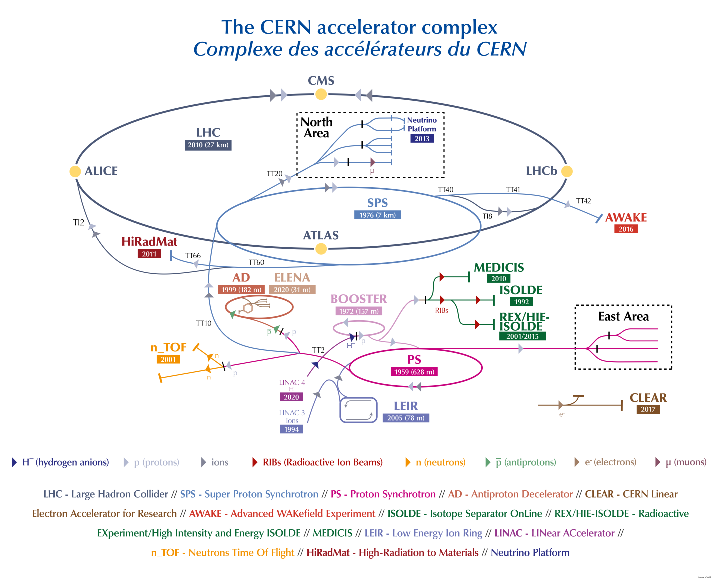
\includegraphics[clip, width=14cm]{fig/2/CCC-v2022.pdf}
  \caption{CERN に設置されている加速器群\cite{article:accelerator-complex}。}
  \label{fig:LHC加速器}
\end{figure}


LHCでは陽子を衝突させるまでに、いくつかの前段加速器を使用しTeVスケールのエネルギーまで陽子を加速している。図\ref{fig:LHC加速器}に概略図を示す。
初めに負水素イオン(H$^-$、水素原子に電子を加えたもの)を線形加速器であるLINAC4\cite{article:Linearaccelerator4}で160~MeVまで加速する。次に、強い電場をかけることで負水素イオンから2個の電子を剥ぎ取り、陽子だけの状態にする。そして、Proton Synchrotron Booster~(PSB)\cite{article:TheProtonSynchrotronBooster}に入射し 1.4~GeVまで加速された後、Proton Synchrotron~(PS)\cite{article:TheProtonSynchrotron}で陽子を26~GeVまで加速し、40~MHzのバンチ構造を持った陽子ビームを形成する。
その後、Super Proton Synchrotron~(SPS)\cite{article:TheSuperProtonSynchrotron}で450~GeVまで加速された後、陽子ビームはLHCに入射され最大で7~TeVまで加速される。
LHCの衝突実験で使用される陽子ビームはバンチと呼ばれる10$^{11}$個の陽子のかたまりで構成されており、LHCの一周あたりに25~nsのバンチ間隔で入射されているため、陽子-陽子衝突を起こす際の各バンチの衝突頻度は40~MHzとなっている。

LHCは陽子ビームが反対方向に周回するための2つのリングから構成されており、4か所ある衝突点にそれぞれ検出器が設置されている。
その衝突点の一つにATLAS検出器が設置され、陽子-陽子衝突から生成される粒子を検出する。
他3箇所にも検出器が設置されており、それぞれCMS~(Compact Muon Solenoid)\cite{article:CMSExperiment}、LHCb~(Large Hadron Collider b)\cite{article:LHCbExperiment}、ALICE~(A Large Ion Collider Experiment)\cite{article:ALICEExperiment}である。
ATLASとCMSの2つの検出器は、標準模型の検証から標準模型を超える現象の探索まで可能な汎用検出器である。
LHCb~と呼ばれる検出器は、B-ハドロン系の物理を研究するために設計されたものである。
最後のALICEは、QCD現象を探るために重イオン衝突の研究に最適化された検出器である。


\section{LHC-ATLAS 実験}\label{section2-2}
本節では、LHC-ATLAS 実験で使用される ATLAS 検出器と ATLAS 実験で使用されているトリガーシステムについて説明する。

\subsection{ATLAS検出器}
ATLAS検出器は、LHCの衝突点の1つに設置された、直径25m、長さ44mの円筒形の大型汎用検出器である\cite{Aad:1129811}。ATLAS 検出器の全体像を図\ref{fig:ATLAS検出器}に示す。
ATLAS検出器は複数の検出器を組み合わせて構成されており、内側から内部飛跡検出器、カロリメータ、ミューオン検出器といった検出器が設置されている。また、内部飛跡検出器とカロリメータの間には超電導ソレノイド磁石、カロリメータの外側にはトロイド磁石がそれぞれ設置されている。
これらの検出器から得られる情報を組み合わせることで、粒子識別や粒子のエネルギーなどの測定を行っている。
以下では各検出器の概要について述べる。

\begin{figure}[tb]
  \centering
  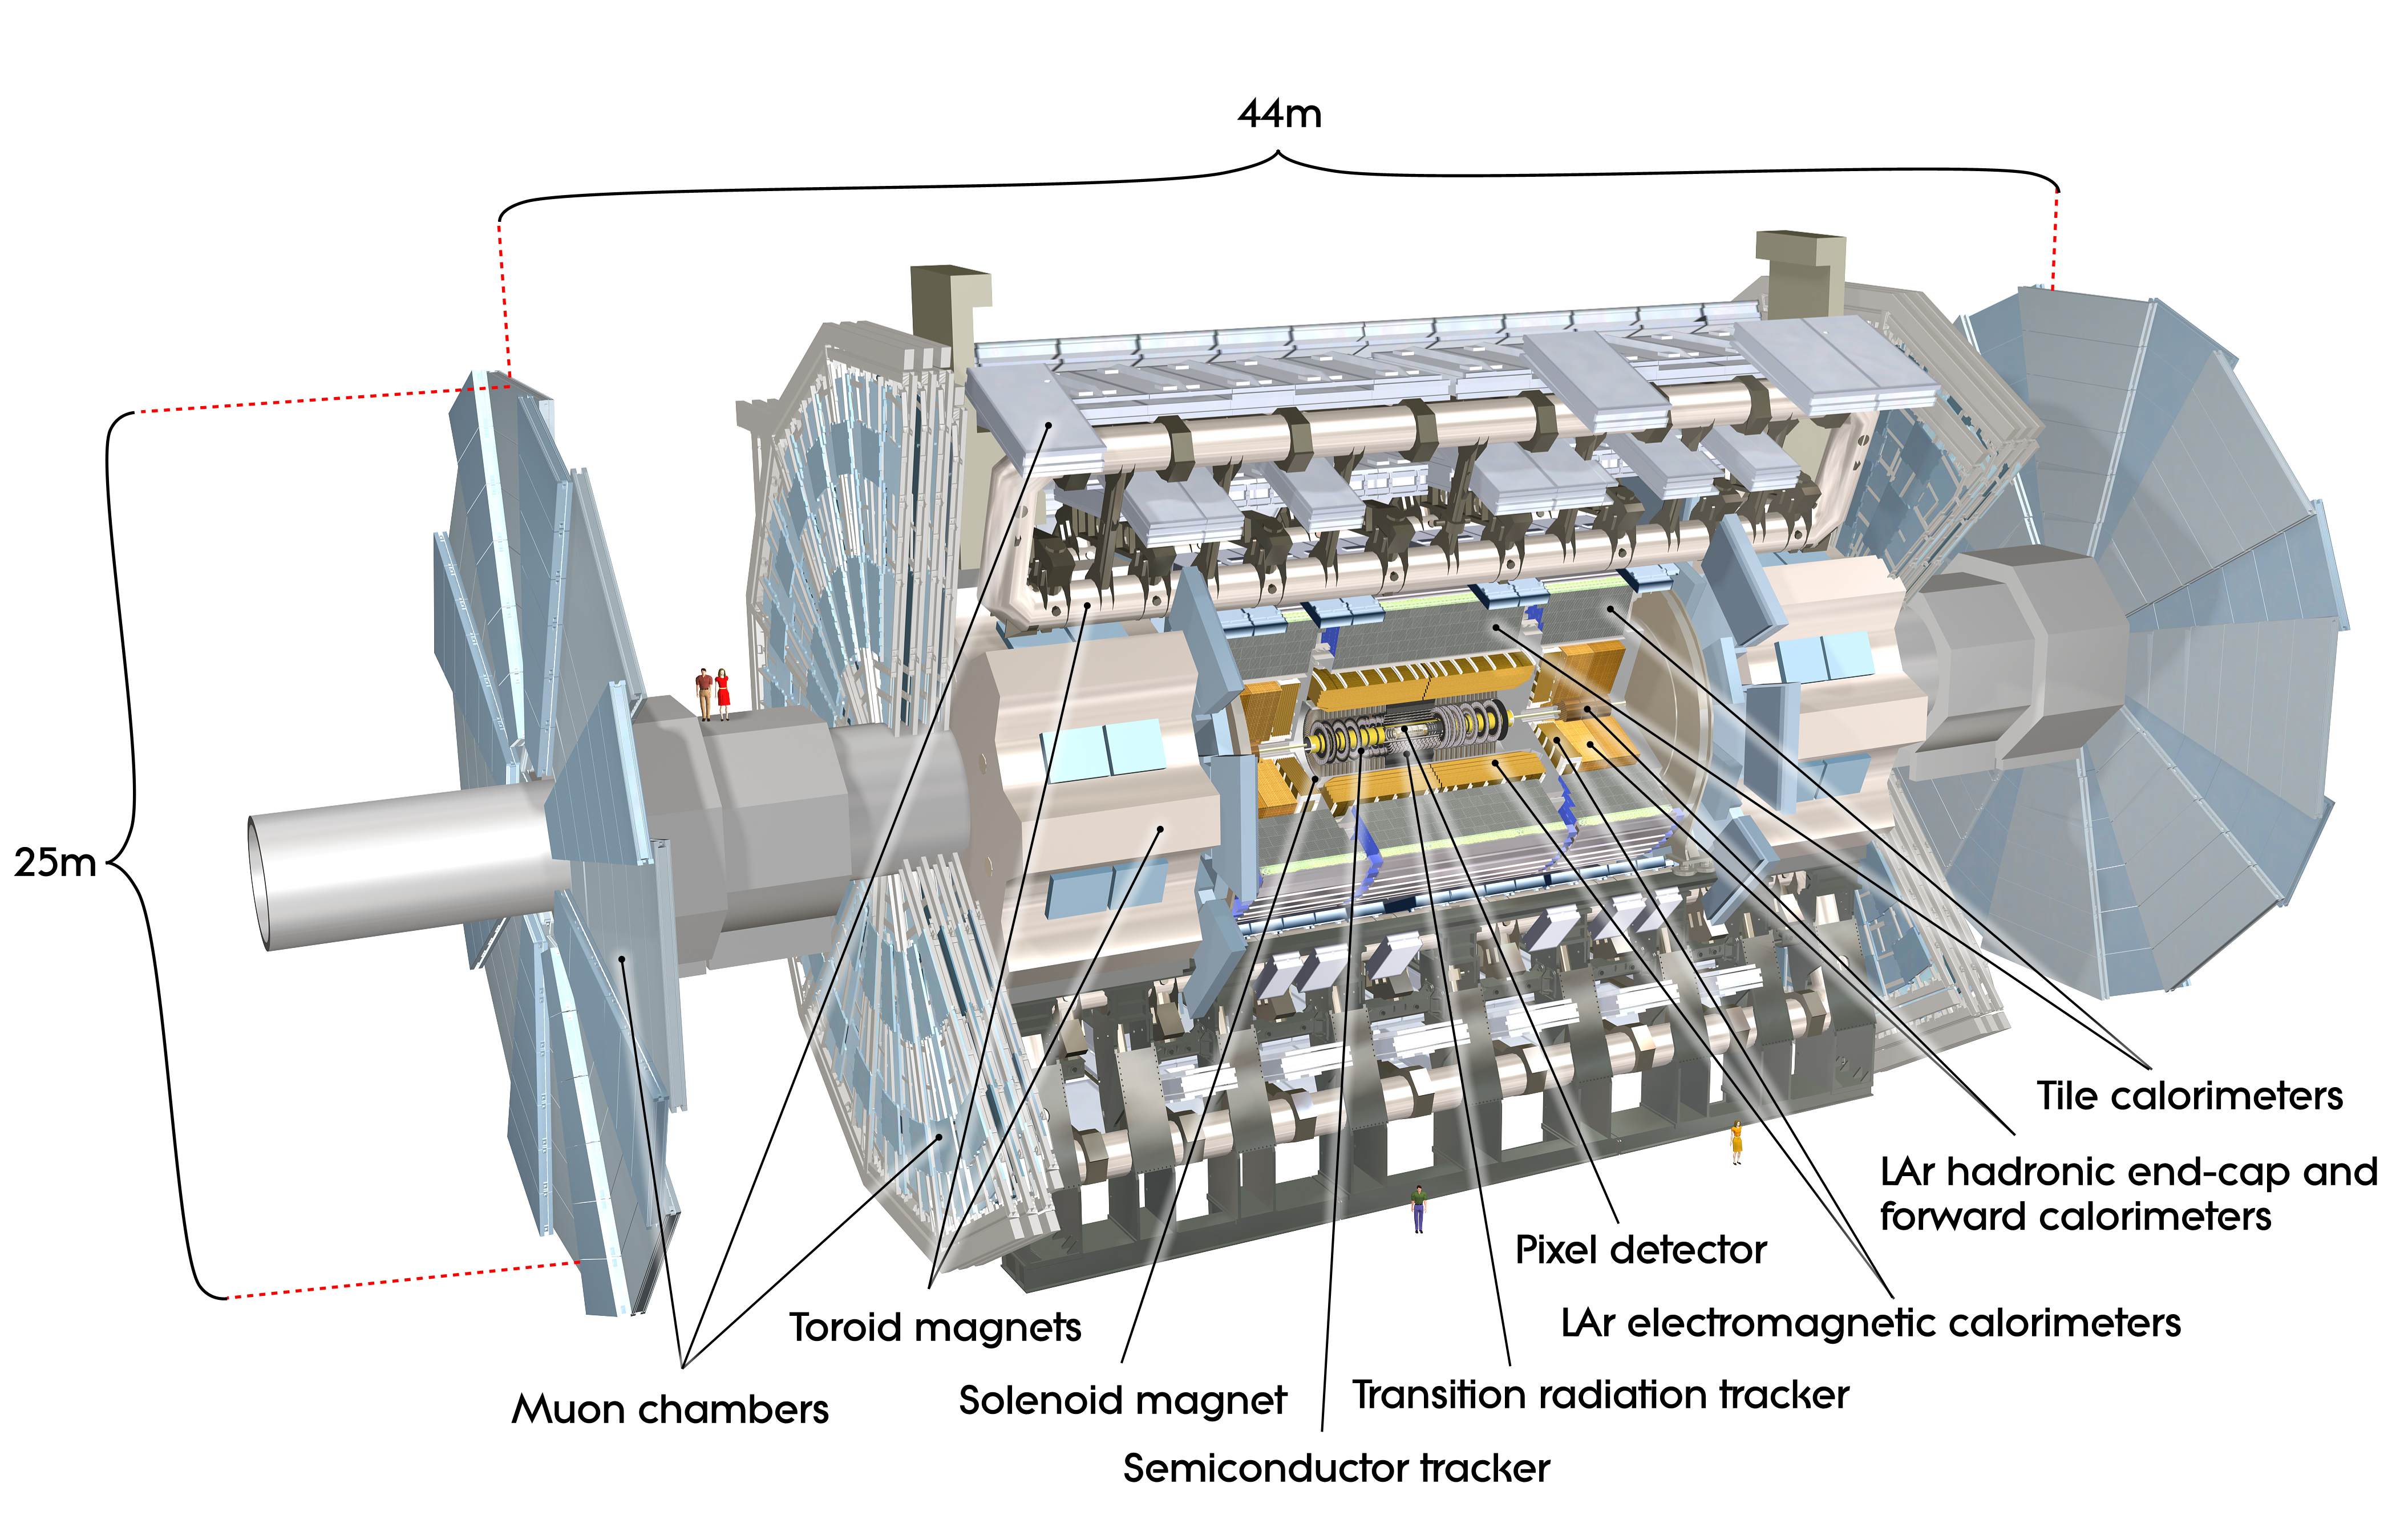
\includegraphics[clip,width=14cm]{fig/2/0803012_01.jpg}
  \caption{ATLAS検出器の全体図\cite{Aad:1129811}。}
  \label{fig:ATLAS検出器}
\end{figure}

\subsection{ATLAS検出器における座標系}
ATLAS実験では図\ref{fig:a}に示すような直行座標系と円筒座標系が使用されている。直行座標系では、検出器の中心を原点として、ビーム軸に沿ってz軸を取る。ビーム軸に垂直な平面をxy平面としたときに、加速器の中心方向を正とするx軸及び、地面に対して垂直方向上向きを正とするy軸を設定する。円筒座標系では、ビーム軸に沿ったz軸に対し、動径方向を$R$、ビーム軸周りの角度を方位角$\phi$、ビーム軸からの角度を極角$\theta$としている。
ATLAS 検出器ではz軸が正の側を A-side、負の側を C-side と定義している。

また、ATLAS実験で使用される座標系として、
\begin{equation}
 \eta=-\ln(\tan\frac{\theta}{2})
 \label{ラピディティ}
\end{equation}
と定義される擬ラピディティ$\eta$が用いられる。

ATLAS 検出器は円筒形をしており、$|\eta| < 1.0$ の側面部分をバレル領域、$|\eta| > 1.0$ の底面部分をエンドキャップ領域と呼ぶ。

\begin{figure}[tb]
  \centering
  \includegraphics[clip, width=11cm]{fig/2/atlas_coordinate_fix.pdf}
  \caption{ATLAS検出器における座標系}
  \label{fig:a}
\end{figure}

\subsection{マグネットシステム}\label{magnetic_filed}
ATLAS 実験では、荷電粒子の運動量測定のために超伝導磁石を用いて磁場をかけている。超伝導磁石は2種類あり、一方は衝突点付近で発生した荷電粒子の運動量測定のために用いられるソレノイド磁石、もう片方はミューオンの運動量測定のために用いられるトロイド磁石である。
図~\ref{fig:磁石}にATLAS検出器に設置されている超電導磁石の配置を示す。
ソレノイド磁石は内部飛跡検出器とカロリメータの間に設置されており、この電磁石が作り出す磁場によって荷電粒子を曲げ、内部飛跡検出器でその曲率を測定することによって横方向運動量を測定する。
トロイド磁石はバレル部とエンドキャップ部に分けられ、それぞれ$\phi$方向に8つずつ等間隔で配置されており、トロイド磁石が作り出す磁場によってミューオンを曲げ、その横方向運動量を測定するために設置されている。
トロイド磁石によって生じる磁場の$\eta$分布を図~\ref{fig:磁場eta}に、xy平面での磁場の分布を図~\ref{fig:磁場平面} に示す。

\begin{figure}[tb]
  \centering
  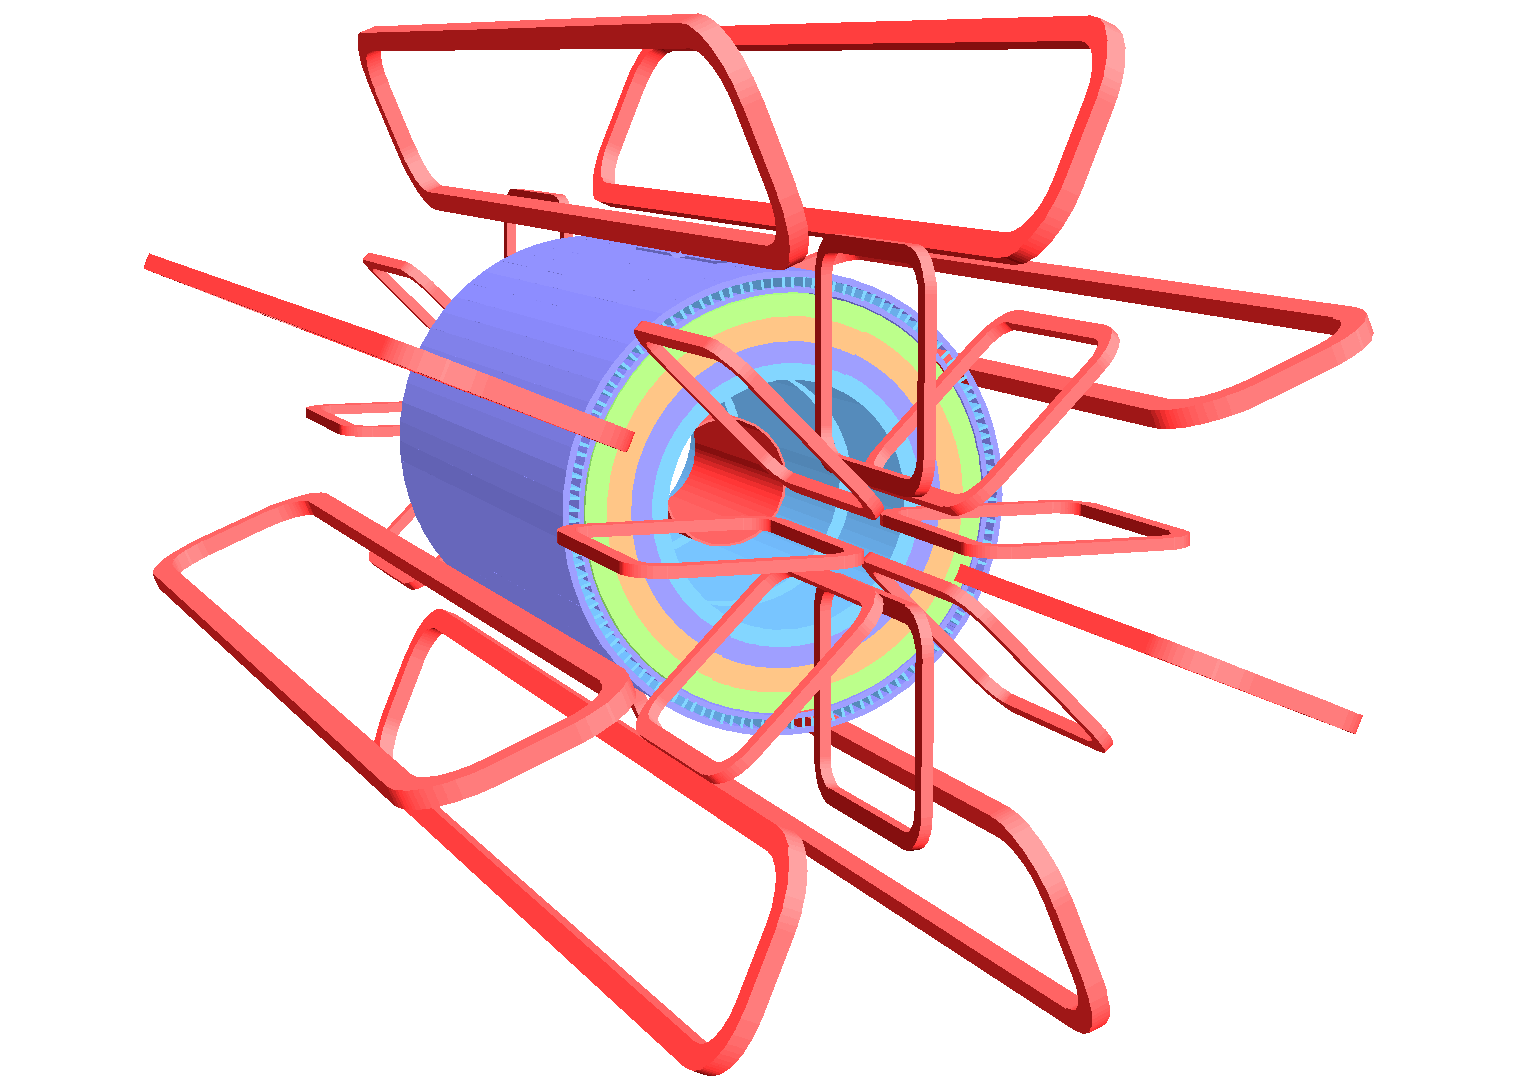
\includegraphics[clip, width=14cm]{fig/2/ATLcoilGeom.pdf}
  \caption{ATLAS検出器で用いられる超電導磁石の配置\cite{Aad:1129811}。}
  \label{fig:磁石}
\end{figure}

\begin{figure}
    \centering
    \begin{minipage}[b]{0.4\linewidth}
        \centering
        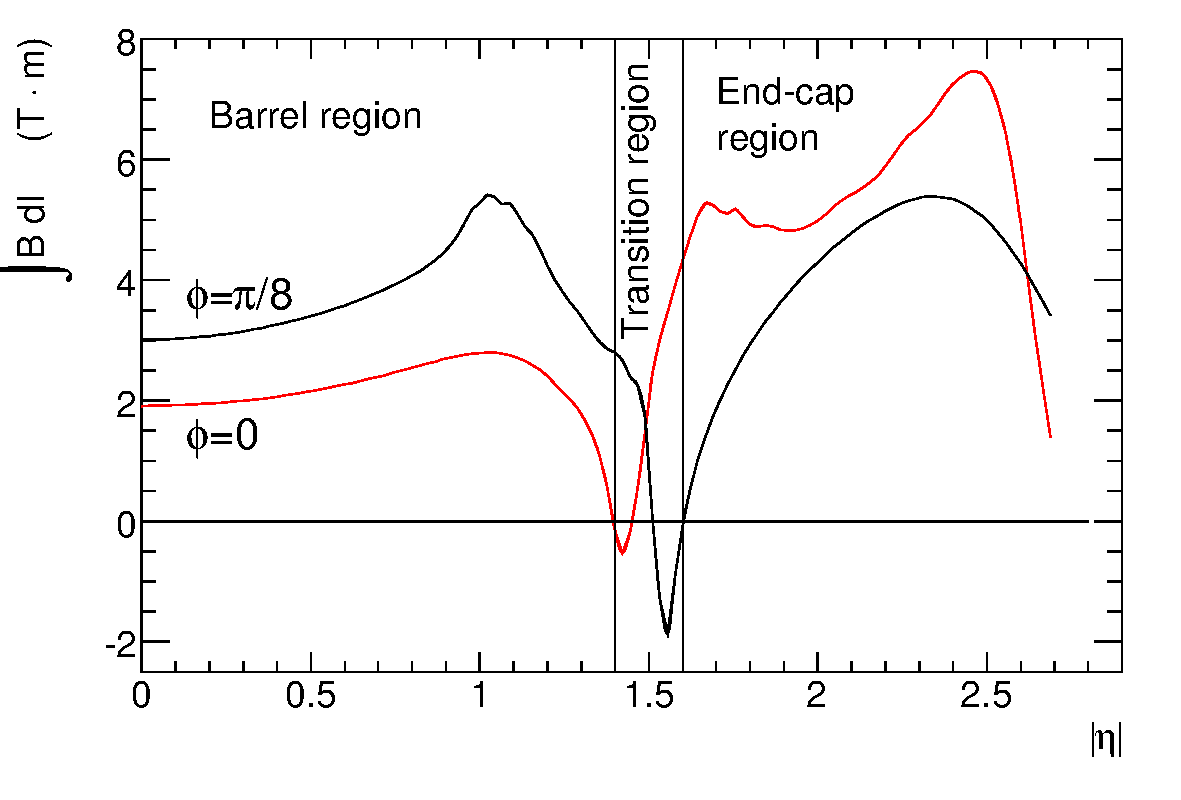
\includegraphics[clip, width=7cm]{fig/2/IBdl.pdf}
        \vspace{10pt}
        \subcaption{}
        \label{fig:磁場eta}
    \end{minipage}
    \hfill
    \begin{minipage}[b]{0.5\linewidth}
        \centering
        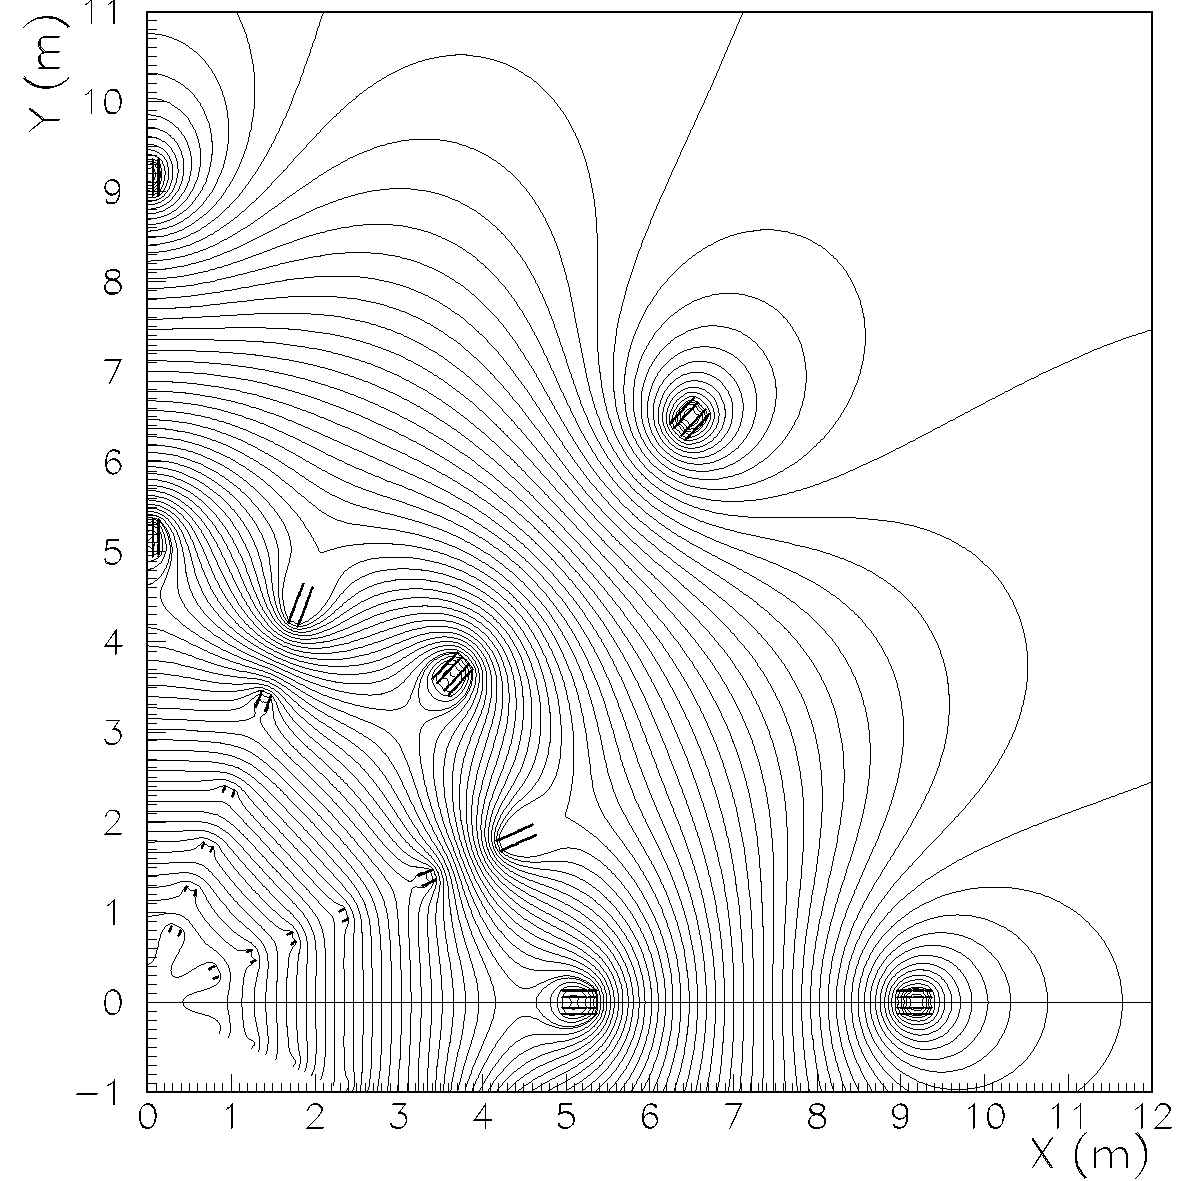
\includegraphics[clip, width=6cm]{fig/2/FMBmap.pdf}
        \vspace{10pt}
        \subcaption{}
        \label{fig:磁場平面}
    \end{minipage}
    \caption{(a):トロイド磁石による磁場の$\eta$分布\cite{Aad:1129811}と、(b):ビーム軸から見た $x − y$ 平面での磁場の分布\cite{article:ATLASMagneticField}。磁石の設置位置の影響により磁場構造が一様ではない。}
    \label{fig:磁場}
\end{figure}




\subsection{内部飛跡検出器}
内部飛跡検出器はビーム衝突点に最も近い位置に設置され、衝突点で発生した荷電粒子の飛跡を測定する。内部飛跡検出器は内側からピクセル検出器~(Pixel)、Semiconductor Tracker~(SCT)、Transition Radiation Tracker~(TRT)で構成されている。

Pixel検出器は最内層にある半導体検出器であり、高い位置分解能を持つ\cite{Aad:1129811}。
SCT はマイクロストリップと呼ばれる細長い有感領域をシリコン上に施した半導体検出器である\cite{Aad:1129811}。そしてTRTは半径4~mmのチューブ型検出器であり、飛跡のトラッキングのほかに遷移輻射を利用した電子の同定も行っている。図~\ref{fig:内部飛跡検出器}に内部飛跡検出器の概略図を示す。

\begin{figure}
    \centering
    \begin{minipage}[b]{0.4\linewidth}
        \centering
        \includegraphics[clip, width=7cm]{fig/2/inner_detectoer1.jpg}
        \vspace{10pt}
        \subcaption{}
        \label{fig:内部飛跡検出器の概略図1}
    \end{minipage}
    \hfill
    \begin{minipage}[b]{0.5\linewidth}
        \centering
        \includegraphics[clip, width=6cm]{fig/2/inner_detector2.jpg}
        \vspace{10pt}
        \subcaption{}
        \label{fig:内部飛跡検出器の概略図2}
    \end{minipage}
    \caption{内部飛跡検出器の全体像及び断面図。(a): 全体像\cite{Aad:1129811}、(b): バレル部の断面図\cite{Collaboration:2723878}。内側から順に Pixel, SCT, TRT 検出器が設置されている。}
    \label{fig:内部飛跡検出器}
\end{figure}



\subsection{カロリメータ}
カロリメータは、内部飛跡検出器の外側に設置されており、LHCでの陽子衝突で生成された粒子のエネルギー及び位置を測定する役割を担っている。
図~\ref{fig:カロリメータ}にATLAS検出器で用いられるカロリメータの概略図を示す。
ATLAS検出器に設置されているカロリメータは、吸収層と検出層からなるサンプリングカロリメータであり、高密度物質の吸収層で粒子シャワーを起こし、検出層で電気信号に変えることで粒子の同定を行っている。
ATLASのカロリメータは、電磁カロリメータとハドロンカロリメータの2種類設置されている。

\begin{figure}[tb]
  \centering
  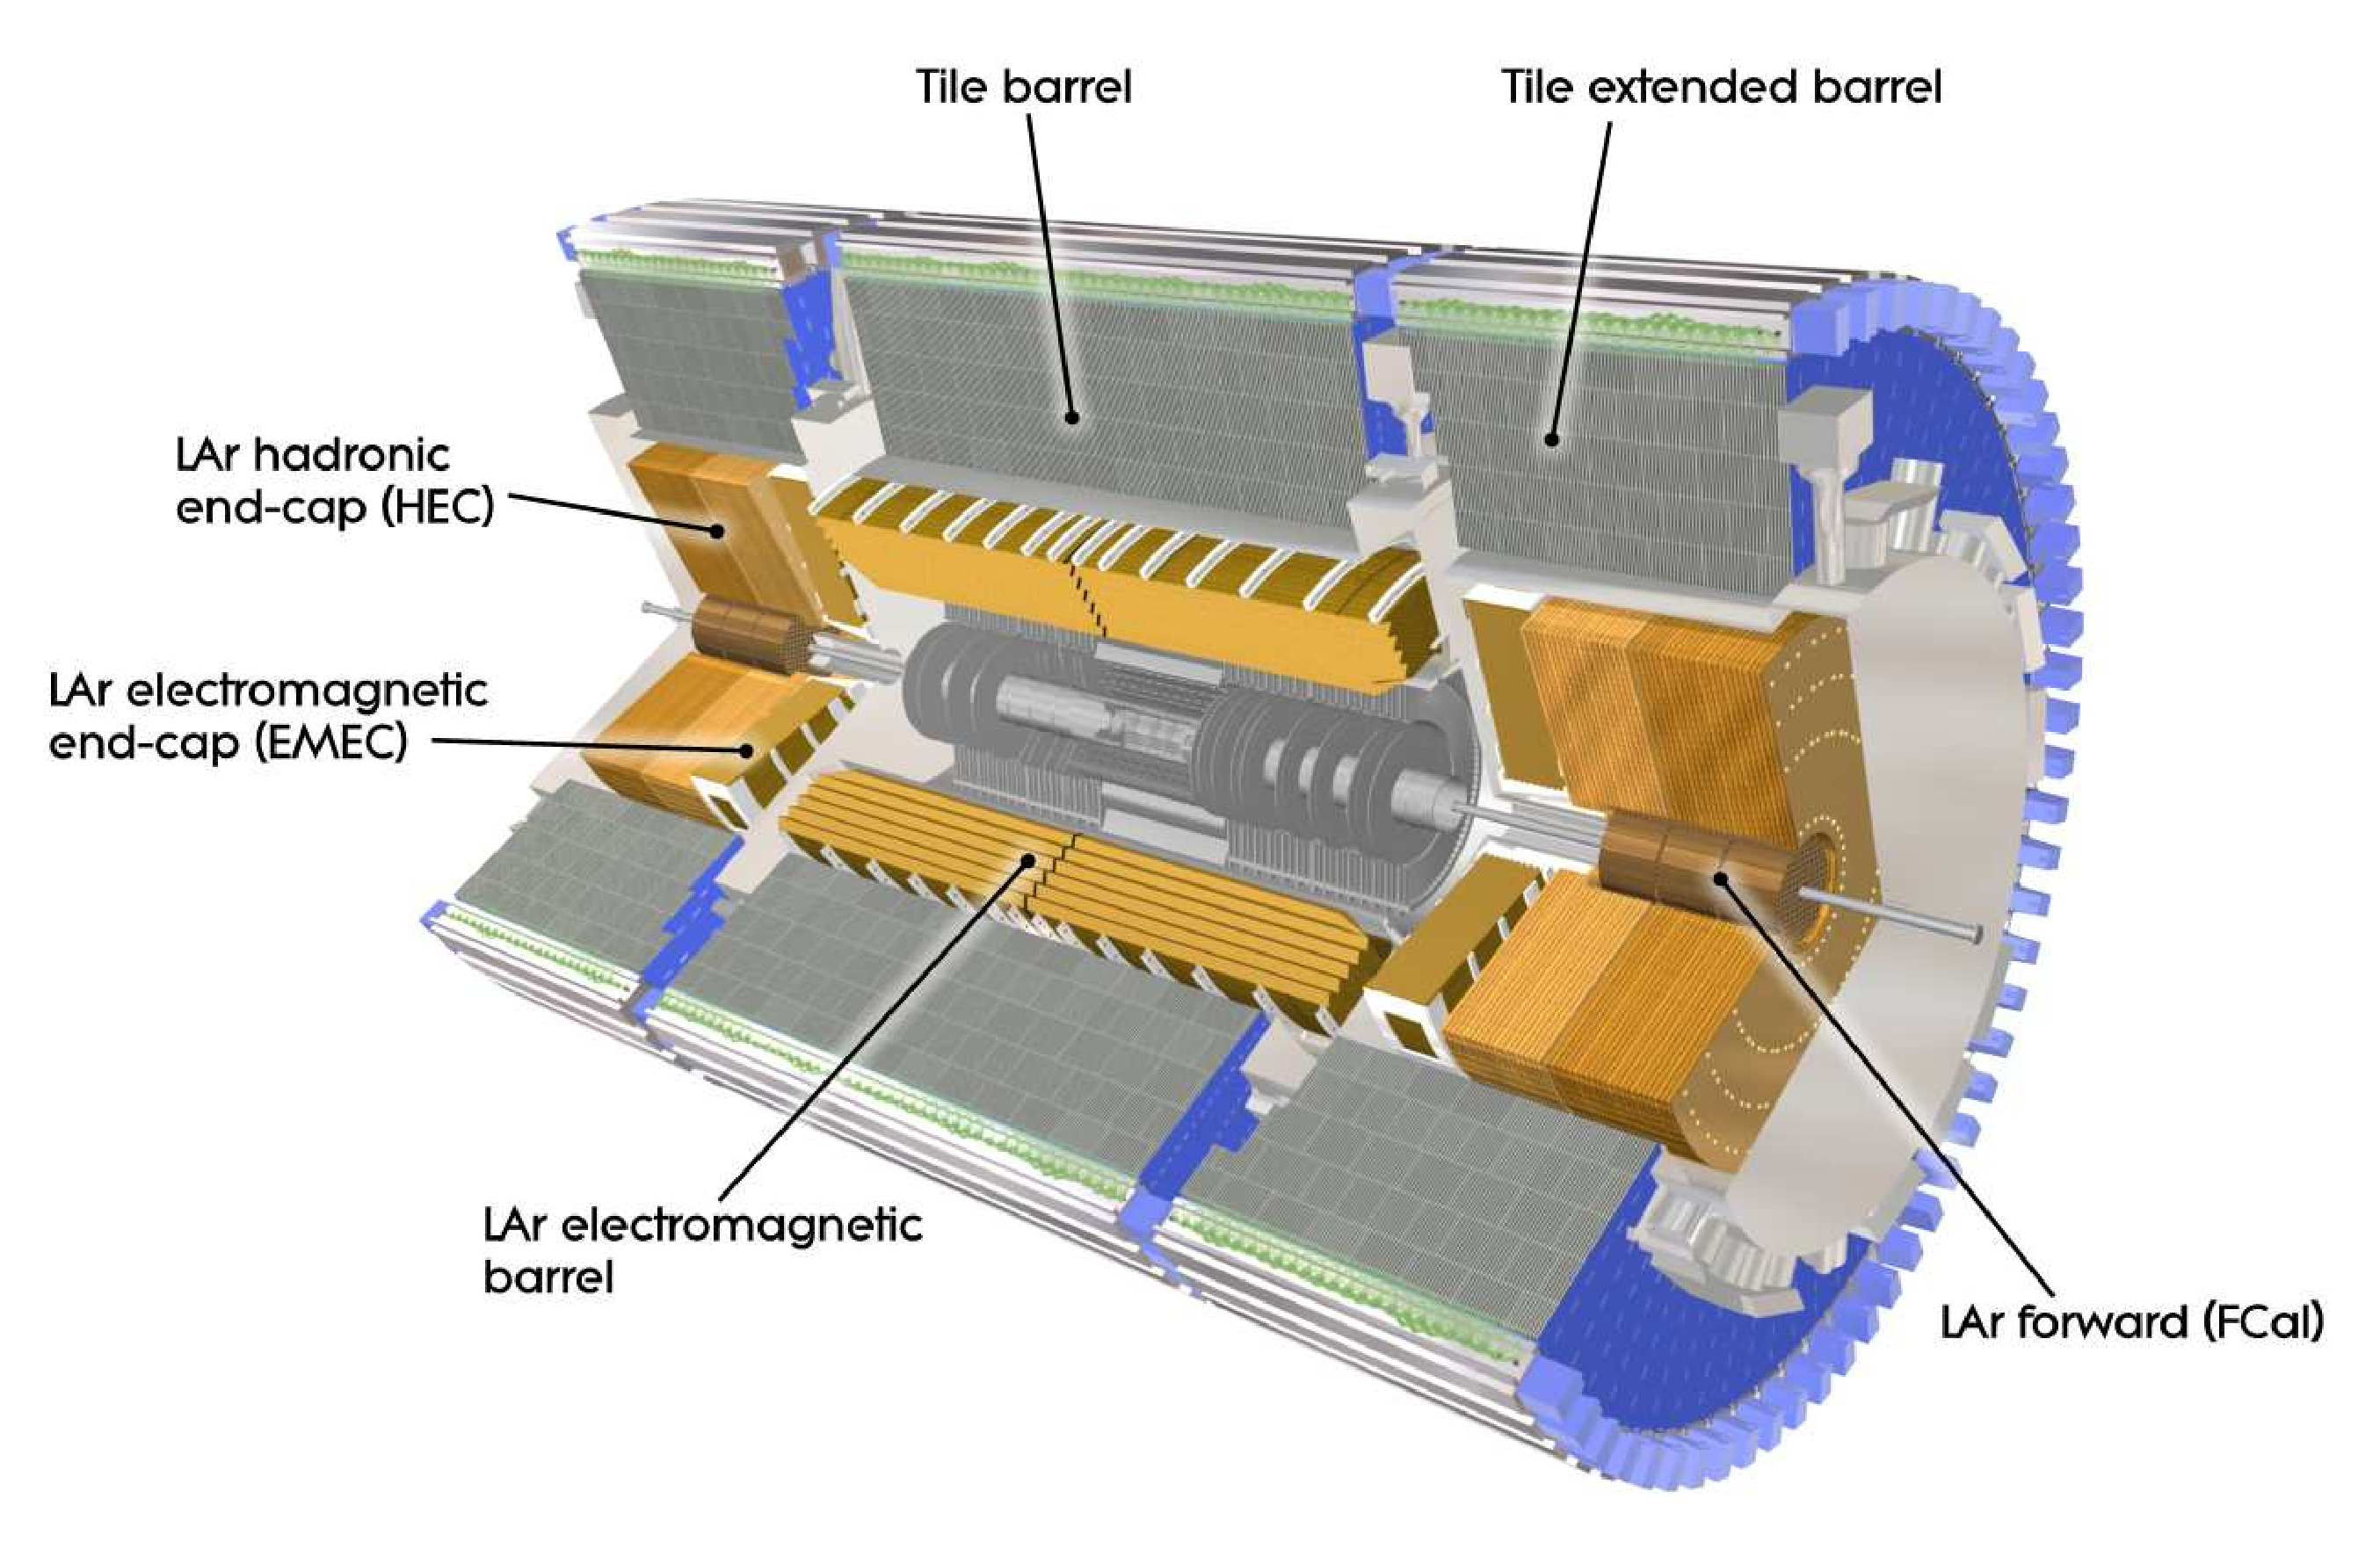
\includegraphics[clip, width=11cm]{fig/2/Calorimeter_d3.pdf}
  \caption{ATLAS 検出器におけるカロリメータの構成\cite{Aad:1129811}。電磁カロリメータは、バレル領域およびエンドキャップ領域の 2 種類。ハドロンカロリメータは、バレル領域のタイル、エンドキャップ領域、フォワード領域の液体アルゴンカロリメータの 3 種類。}
  \label{fig:カロリメータ}
\end{figure}

\subsubsection{電磁カロリメータ}
電磁カロリーメーターは、$|\eta|<1.5$をカバーするバレルカロリメータと、$1.4<|\eta|<3.4$をカバーするエンドキャプカロリメータに分かれている。
バレル部とエンドキャプ部ともに、吸収層の鉛と検出層の液体アルゴンで構成されたカロリメータであり、電磁相互作用を起こす光子や電子のエネルギーと位置を測定する役割を担っている。

\subsubsection{ハドロンカロリメータ}
ハドロンカロリメータは電磁カロリメータの外側に設置されており、タイルカロリーメータ、エンドキャップカロリーメータ、フォワードカロリーメータの3つに分類され、それぞれ異なる$\eta$の範囲をカバーする。バレル部では、鉄の吸収体とタイル状のシンチレータから構成されたタイルカロリメータが設置されている。エンドキャプ部では、銅の吸収体と液体アルゴンから構成されたエンドキャプカロリメータが使用されている。さらに、フォワード領域では銅とタングステンの吸収体と液体アルゴンからなるフォワードカロリメータが設置されている。

\subsection{ミューオン検出器}\label{section2-2-4}
ミューオン検出器はATLAS検出器の最外層に設置されており、カロリメータを通過したミューオンを検出するために用いられる。
ミューオン検出器はResistive Plate Chamber~(RPC)とThin Gap Chamber~(TGC) という2種類のトリガー検出器と、Monitored Drift Tube~(MDT)とCathode Strip Chamber~(CSC)の2種類の精密測定用の検出器によって構成される。
図~\ref{fig:ミューオン}にミューオン検出器の配置図を示す。

ミューオン検出器は、層状に設置されているステーションと呼ばれる単位で定義される。
エンドキャップ部ではビーム軸に対して垂直に円盤状のステーションを、バレル部では筒状のステーションを構成している。
エンドキャップ、バレル領域において検出器は3層構造であり、衝突点に近い方から Inner(I)、Middle(M)、Outer(O) と呼ぶ。
またミューオン検出器はトロイド磁石と干渉しないように配置するため、$\phi$方向においてはLarge Chamber~(L)とSmall Chamber~(S)の2種類の検出器を組み合わせてステーションを構成している。

\begin{figure}[tb]
  \centering
  %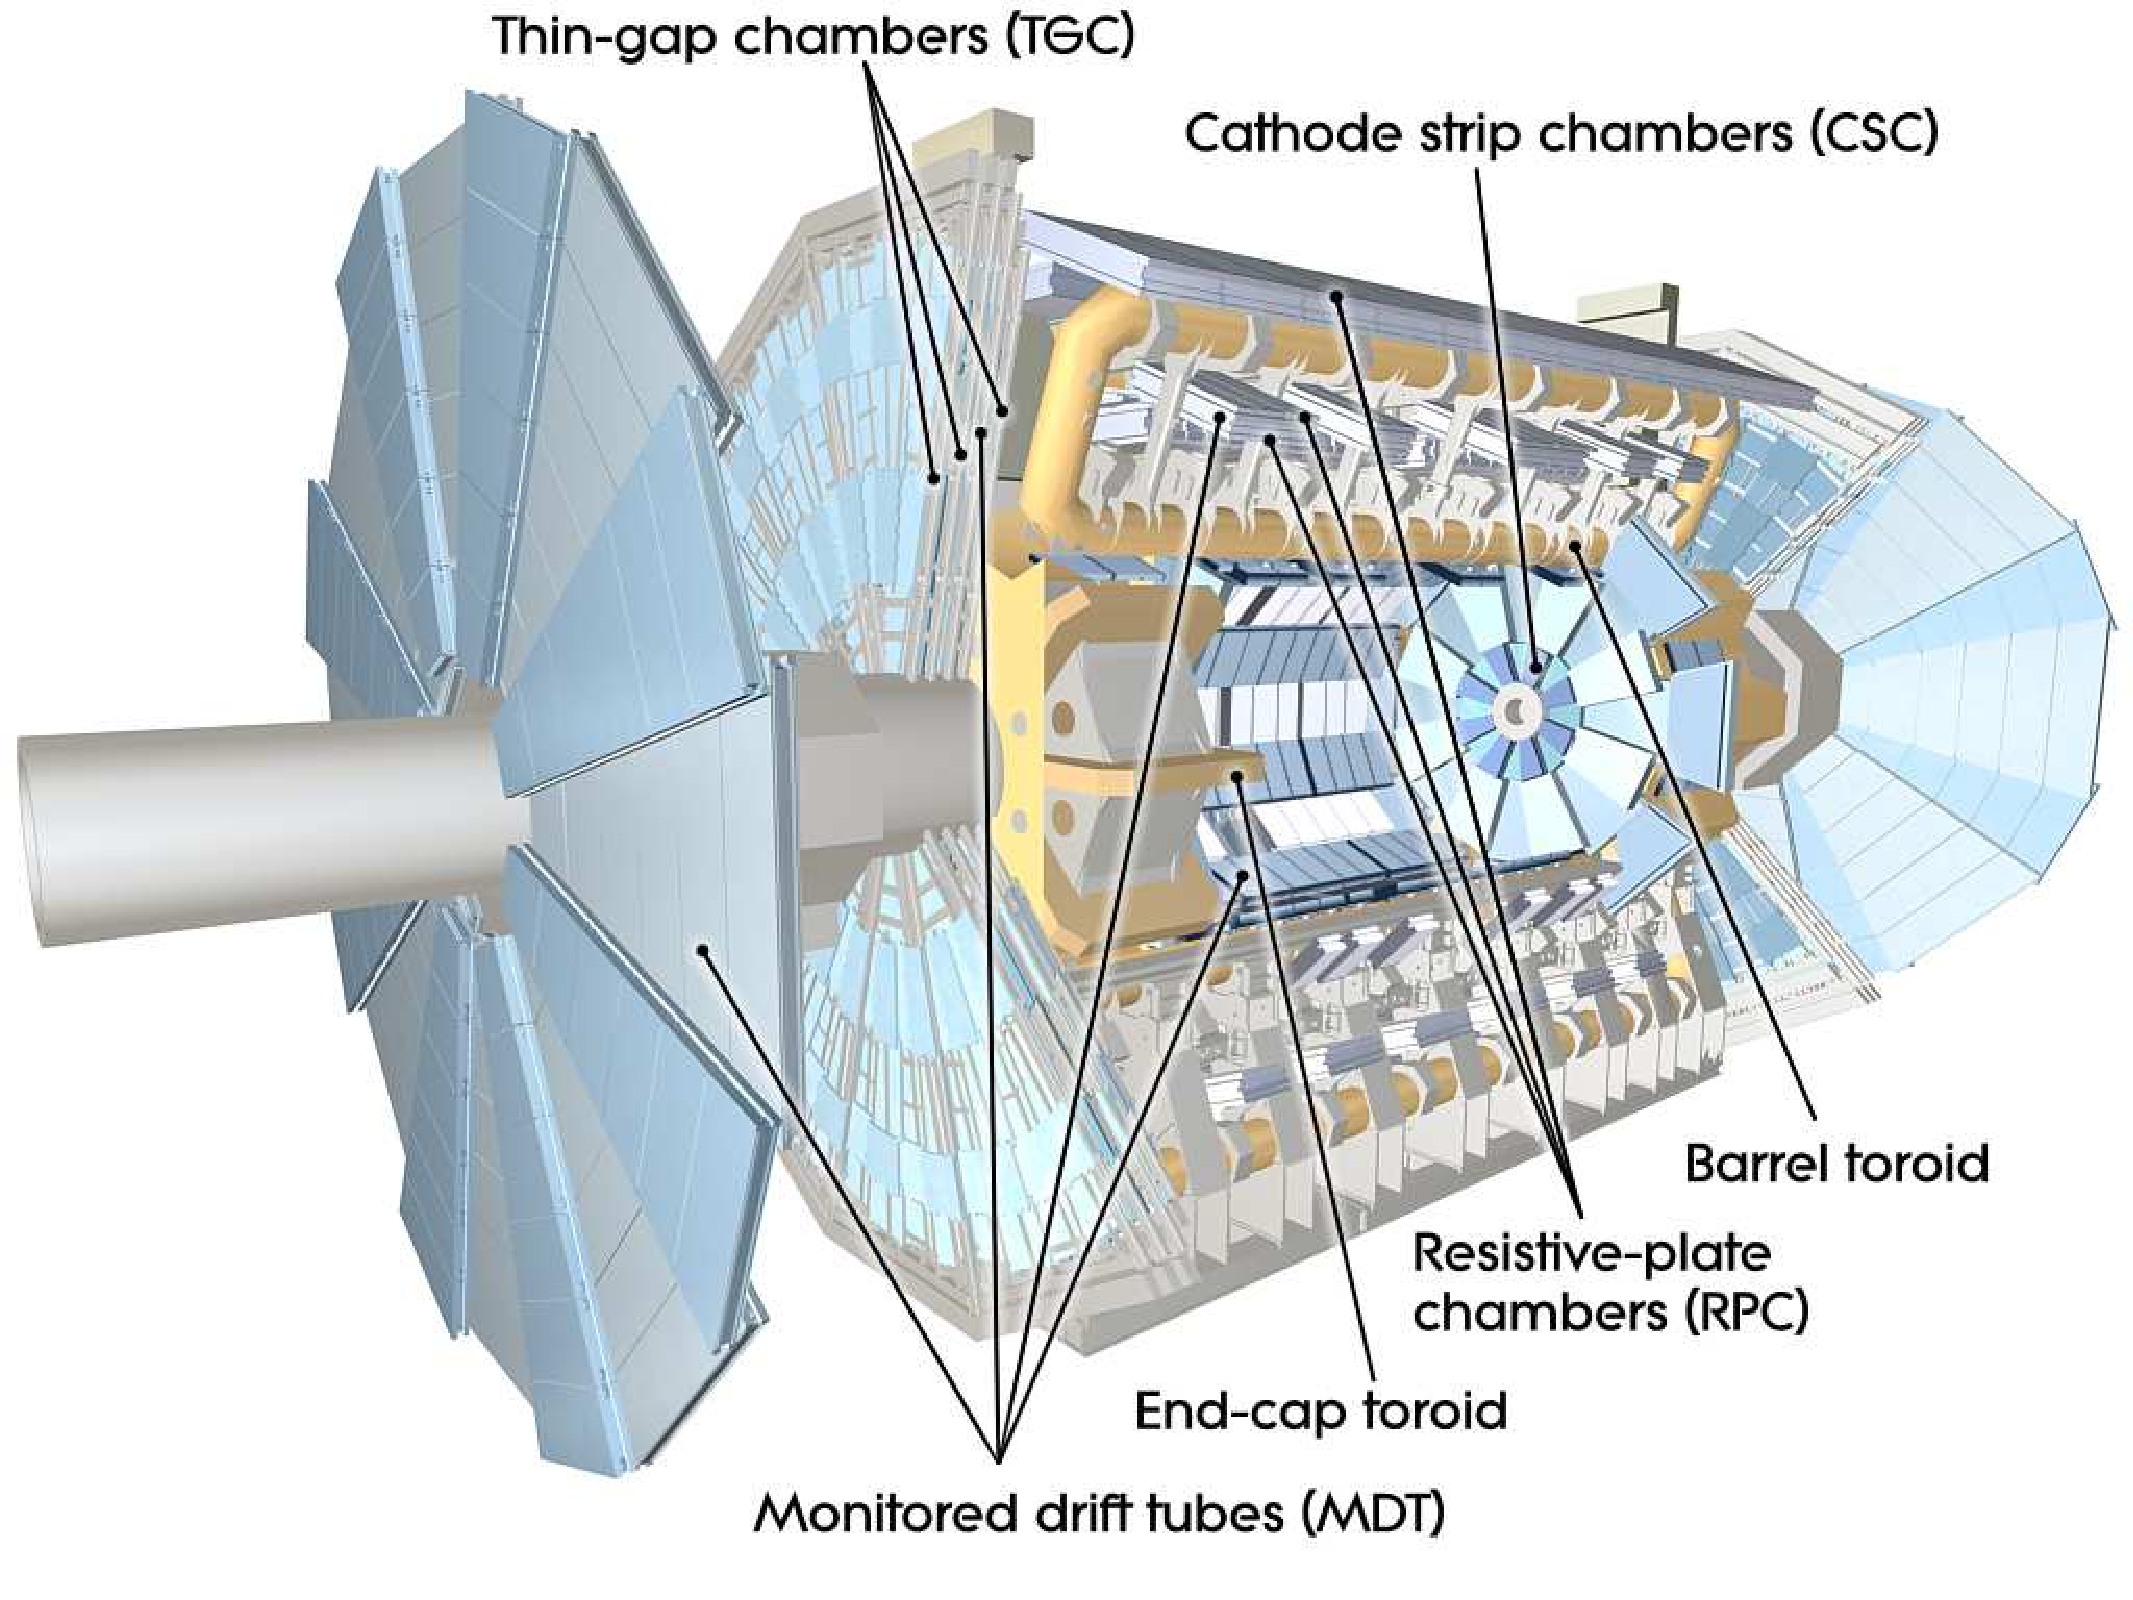
\includegraphics[clip, width=11cm]{fig/2/MuonSystem_d3.pdf}
  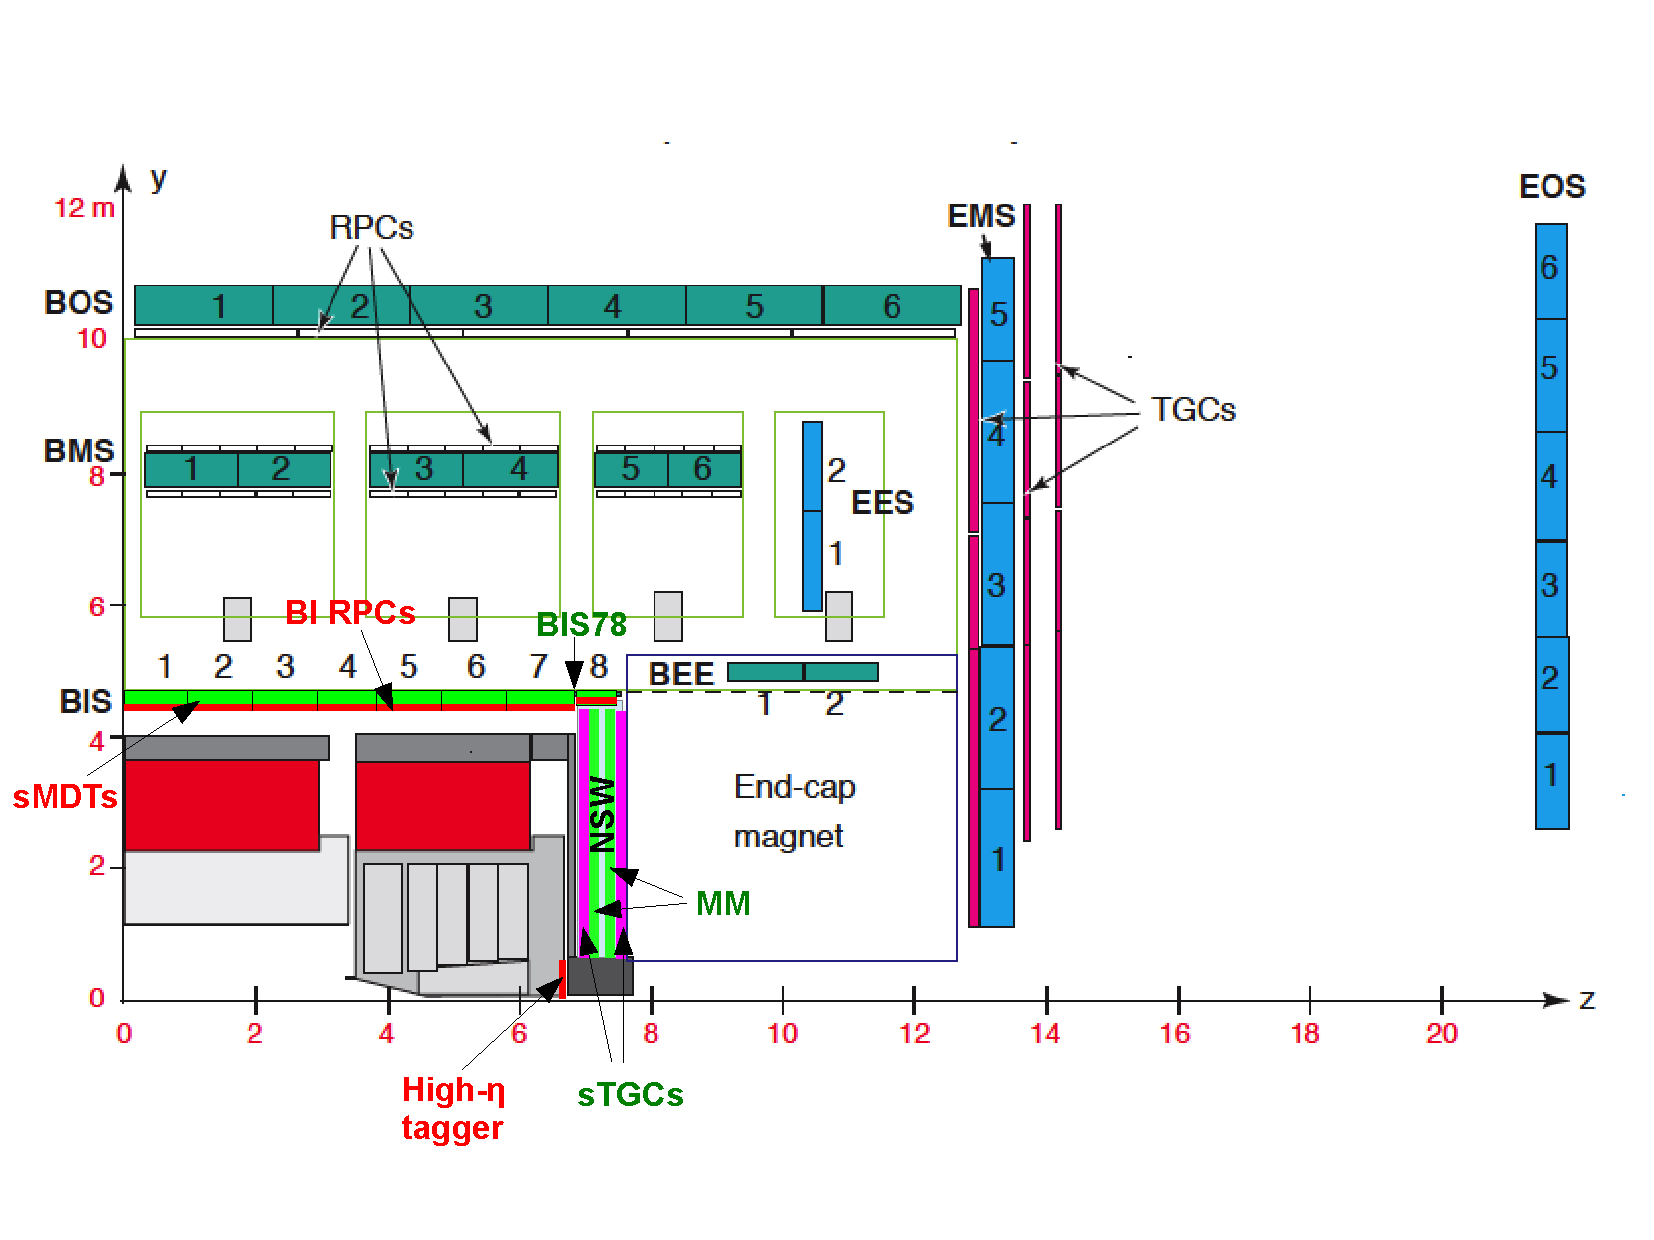
\includegraphics[clip, width=11cm]{fig/2/ch01_fig_03a.pdf}
  \caption{ミューオンスペクトロメータの配置図\cite{article:phase2}。}
  \label{fig:ミューオン}
\end{figure}

\subsubsection{Resisitive Plate Chamber (RPC)}
RPCはバレル部のミューオントリガー判定に用いられるミューオン検出器である。図~\ref{fig:RPC} にRPC検出器の構造を示す。2枚の高抵抗プレートの間に幅2~mmの絶縁体を挟み込んでおり、9.8~kVの高電圧をかけている。各検出器は2層構造になっており、直交するストリップの情報から$\eta$と$\phi$の位置を読み出している。

\begin{figure}[tb]
  \centering
  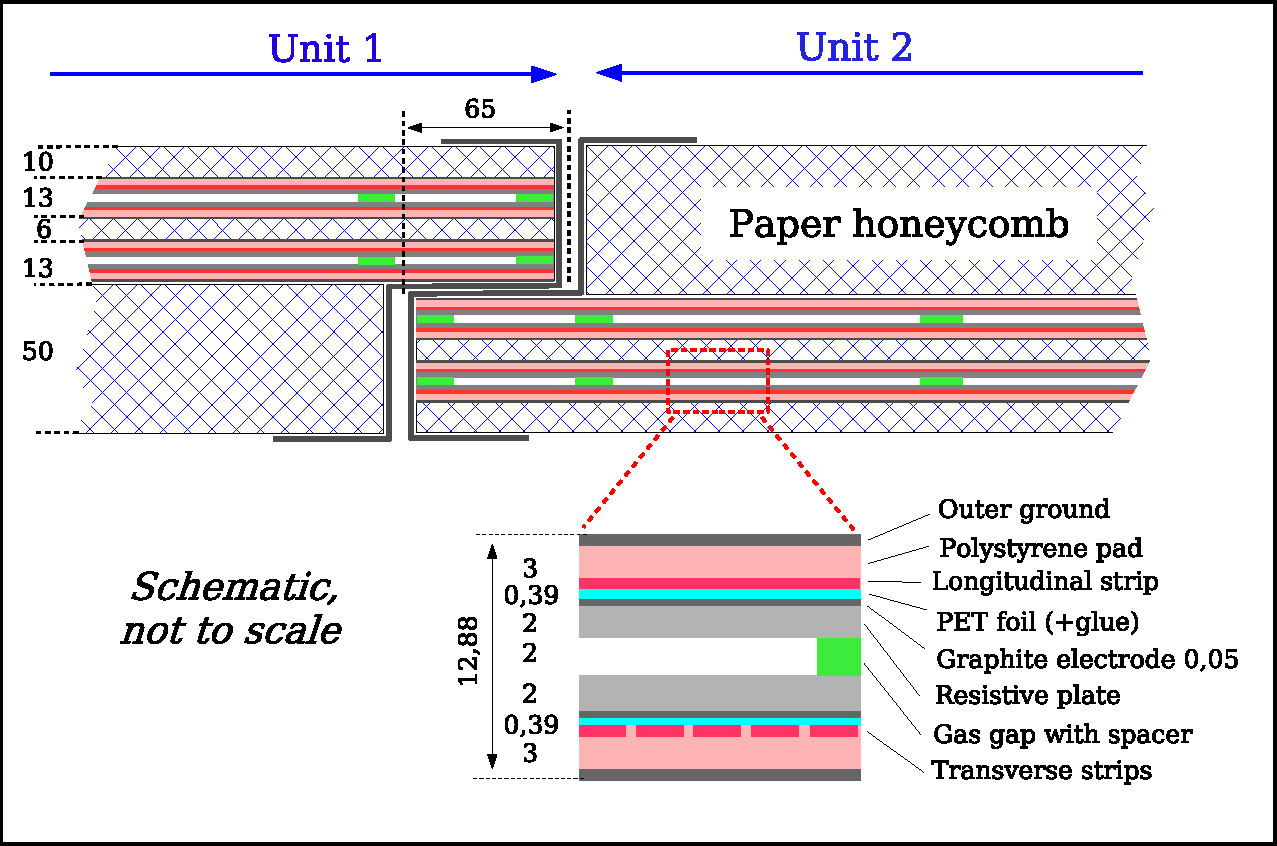
\includegraphics[clip, width=10cm]{fig/2/RPC_structure.pdf}
  \caption{RPCの構造図\cite{Aad:1129811}}
  \label{fig:RPC}
\end{figure}




\subsubsection{Thin Gap Chambers (TGC)}
TGCはエンドキャプ部の$1.05 < |\eta| < 2.7$の領域に設置されているミューオン検出器である。R-z平面における図~\ref{fig:TGC_st}にTGC検出器の配置図を示す。
TGC は Multi Wire Proportional Chamber~(MWPC) の一種で、ワイヤーとストリップによる2 次元読み出しを行うことでミューオンのヒット位置を測定する。図~\ref{fig:MWPC}にTGCの構造を示す。
アノードワイヤーには直径50$\mu$mの金メッキをしたタングステンワイヤーを用い、カソードには片面に表面抵抗1M$\Omega$のカーボンを塗布したガラスエポキシ板を用いている。反対側の面には銅で出来たストリップがワイヤーに直交するように張られている。ミューオンの位置情報のうちRをアノードワイヤーで、$\phi$をカソードストリップで測定することで2次元での読み出しが可能となっている。
図~\ref{fig:TGC}に示すように、TGCを構成する検出器には2層構造のDoubletと3層構造のTripletの2種類がある。
Doubletはワイヤー面2層とストリップ面2層から信号の読み出しを行う。Triplet は3層構造になっているが、真ん中の層にストリップ面はないためワイヤー面3層とストリップ面2層から信号の読み出しを行う。

図~\ref{fig:TGC_st}に示すようにTGC検出器はトロイド磁石による磁場領域より内側にEI~(Endcap Inner)、FI~(Forward Inner)と呼ばれる2つのステーション、磁場領域より外側にM1、M2、M3~(Middle 1,Middle 2,Middle 3)と呼ばれる3つのサブステーションが配置されており、M!、M2、M3の3つのステーションを合わせてTGC Big Wheel~(TGC BW)と呼ぶ。。M1はTriplet構造であり、EI/FI、及びM2、M3はDoublet構造である。
M1、M2、M3は図~\ref{fig:TGC_oc}のように複数のチェンバーを組み合わせた円盤状の検出器である。$1.05 < |\eta| < 1.92$ の領域をエンドキャップ領域、$1.92 < |\eta| < 2.4$ の領域をフォワード領域と呼ぶ。


\begin{figure}[tb]
  \centering
  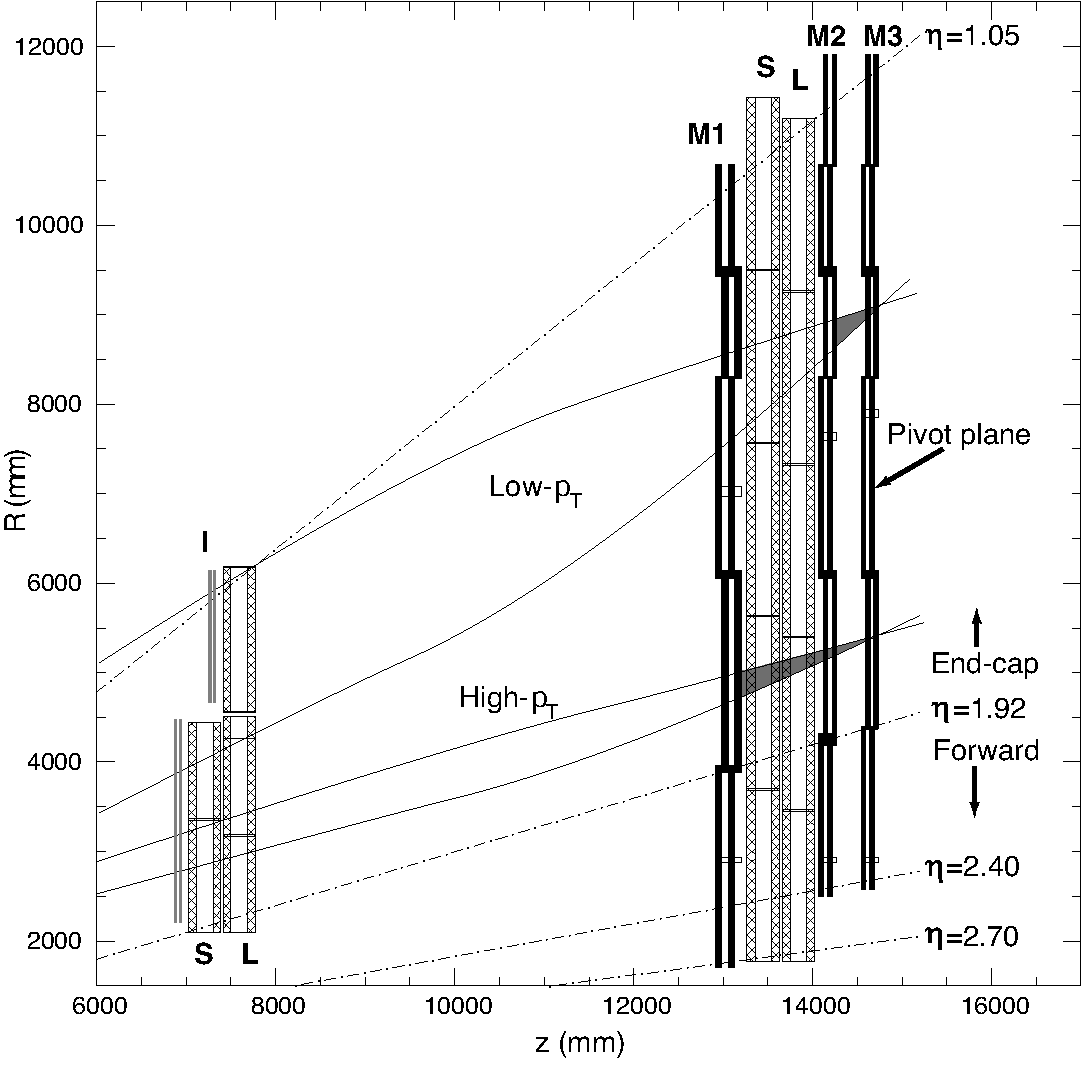
\includegraphics[clip, width=11cm]{fig/2/l1mue-schema.pdf}
  \caption{TGC 検出器の配置図\cite{Aad:1129811}。磁場領域の内側に EI,FI 、外側にTGC-BWと呼ばれる3層のステーション(M1,M2,M3)が設置されている。}
  \label{fig:TGC_st}
\end{figure}

\begin{figure}[tb]
  \centering
    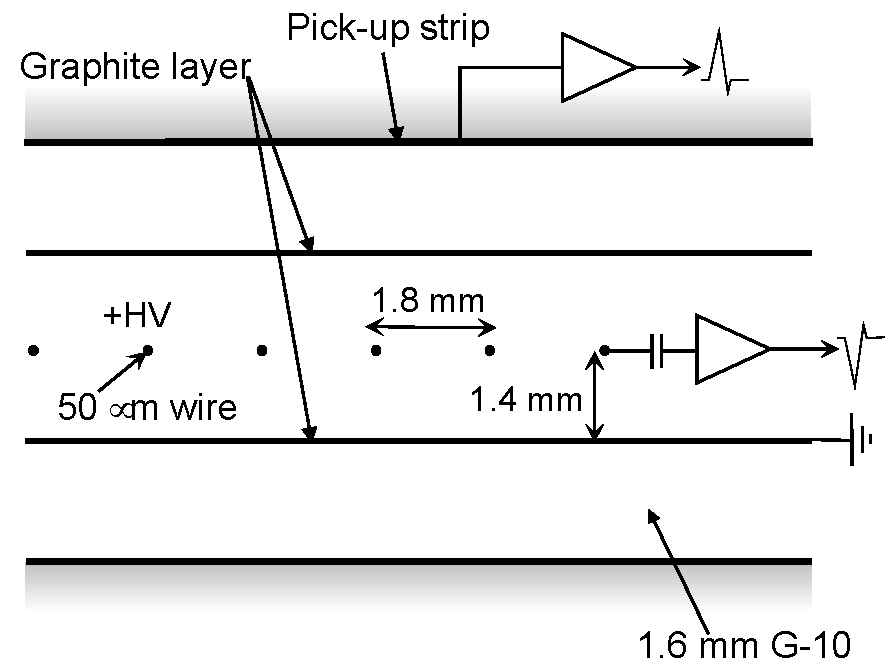
\includegraphics[clip, width=11cm]{fig/2/TGC_anode_wire.pdf}
  \caption{TGC 検出器の構造\cite{Aad:1129811}。ガスギャップ2.8~mm、ワイヤー間隔2.8~mmのMWPC~(Multi
Wired Proportional Chamber)の構造をしている。}
  \label{fig:MWPC}
\end{figure}

\begin{figure}[tb]
  \centering
  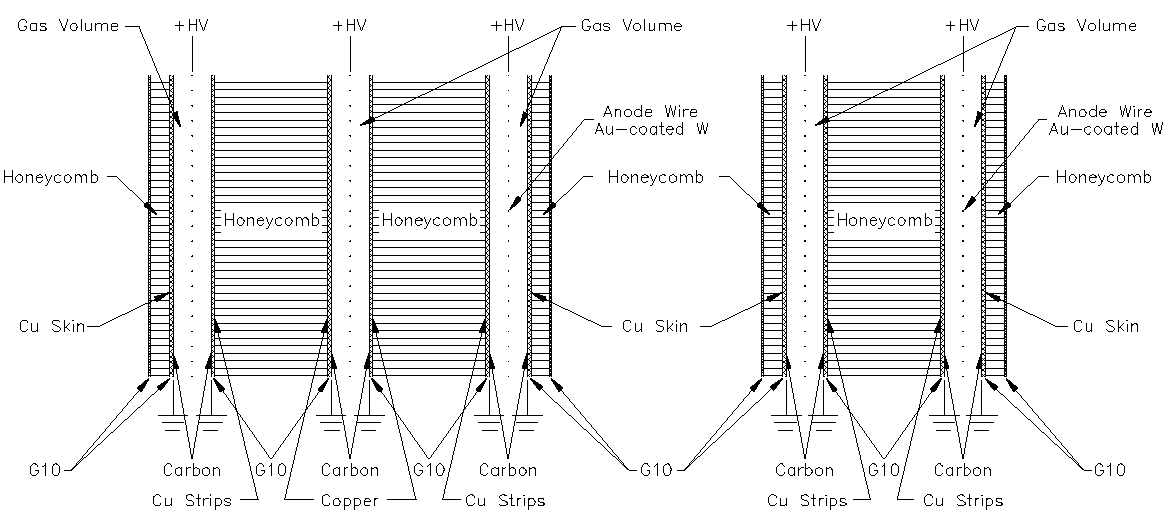
\includegraphics[clip, width=11cm]{fig/2/TGC_construction.pdf}
  \caption{TGC Triplet と Doublet の断面図\cite{Aad:1129811}。}
  \label{fig:TGC}
\end{figure}

\begin{figure}[tb]
  \centering
  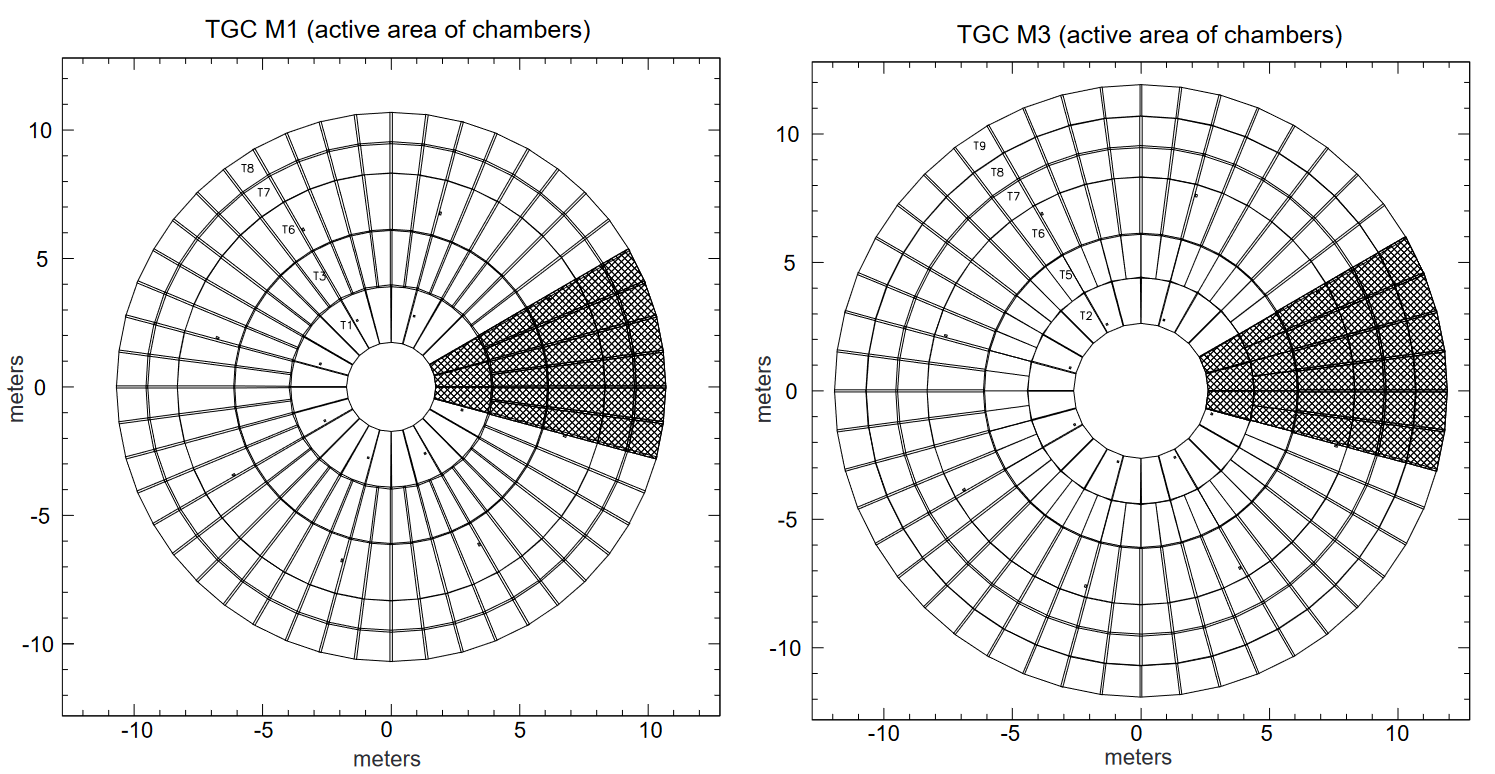
\includegraphics[clip, width=11cm]{fig/2/TGC_octant.png}
  \caption{TGC 検出器 の M1、M3 ステーションの概要図\cite{Lellouch:684103}。実線で囲まれたマスが 1 つのチェンバーに対応する。}
  \label{fig:TGC_oc}
\end{figure}

\subsubsection{Monitored Drift Tube (MDT)}
MDT はミューオンの飛跡の精密測定を目的とした検出器であり、直径約30~mmのドリフトチューブを6層または8層並べた構造をしている。MDTの構造図を図~\ref{fig:MDT} に示す。ドリフトチューブにはアルゴン・二酸化炭素混合ガスを封入している。電離によって生じた電子は、ドリフトチューブの中心に張られている直径50~$\rm{\mu}$m のアノードワイヤーで集められる。


\begin{figure}[tb]
  \centering
  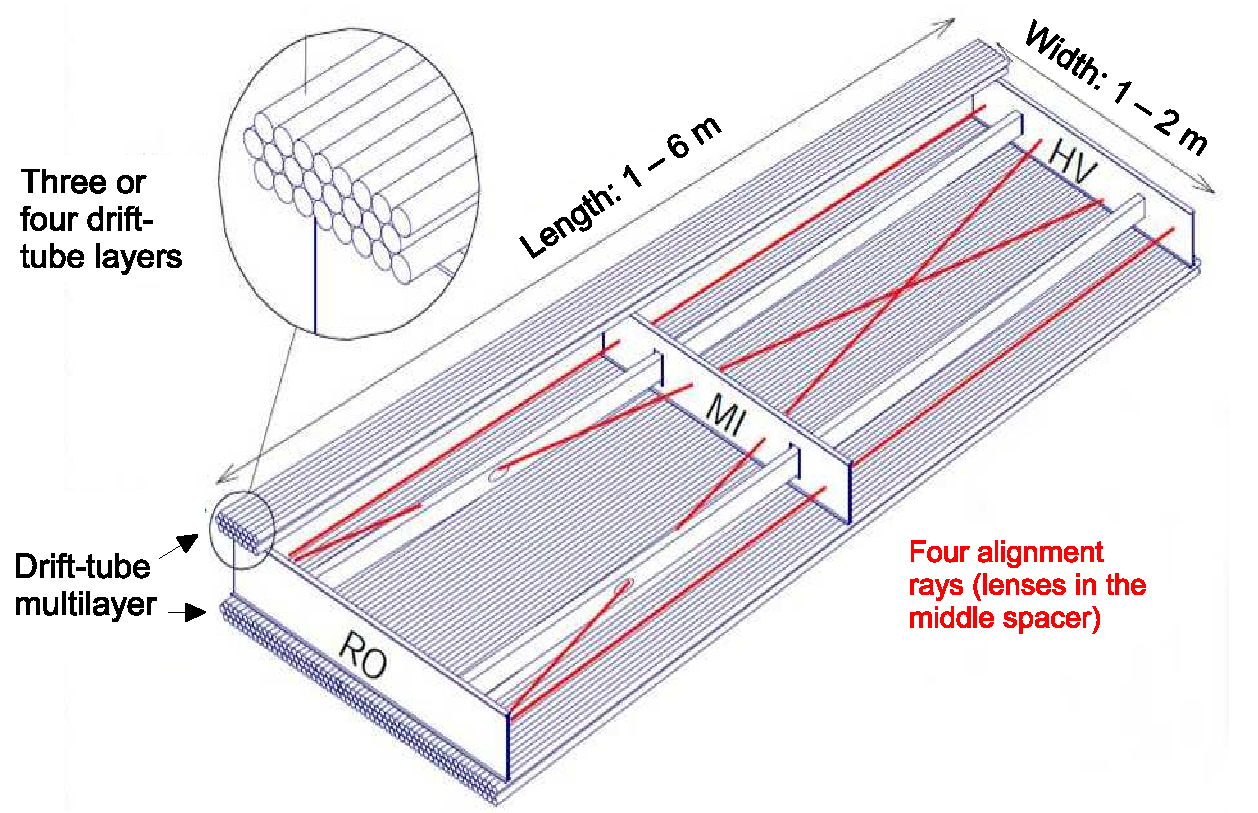
\includegraphics[clip, width=11cm]{fig/2/MDT_chamber_schematics_2.pdf}
  \caption{MDT の構造図\cite{Aad:1129811}。ドリフトチューブを積み重ねたような構造となっている。}
  \label{fig:MDT}
\end{figure}


\subsubsection{New Small Wheel (NSW)}
New Small Wheel~(NSW) は高ヒットレート環境での飛跡測定効率の向上とミューオントリガーの改良を目的として、エンドキャップ部の磁場領域より内側にRun-3から導入された検出器である。図~\ref{fig:NSW}にNSWの全体像を示す。
NSWはエンドキャプ領域の$1.3 < |\eta| < 2.7$ の全$\phi$領域を覆うように設置されており、small-strip TGC~(sTGC)とMicromegas~(MM) の2種類の検出器を4層ずつ組み合わせた構造をしている。このため、NSWからは位置情報だけでなく飛跡の再構成による角度情報も得ることができる。

\begin{figure}[tb]
  \centering
  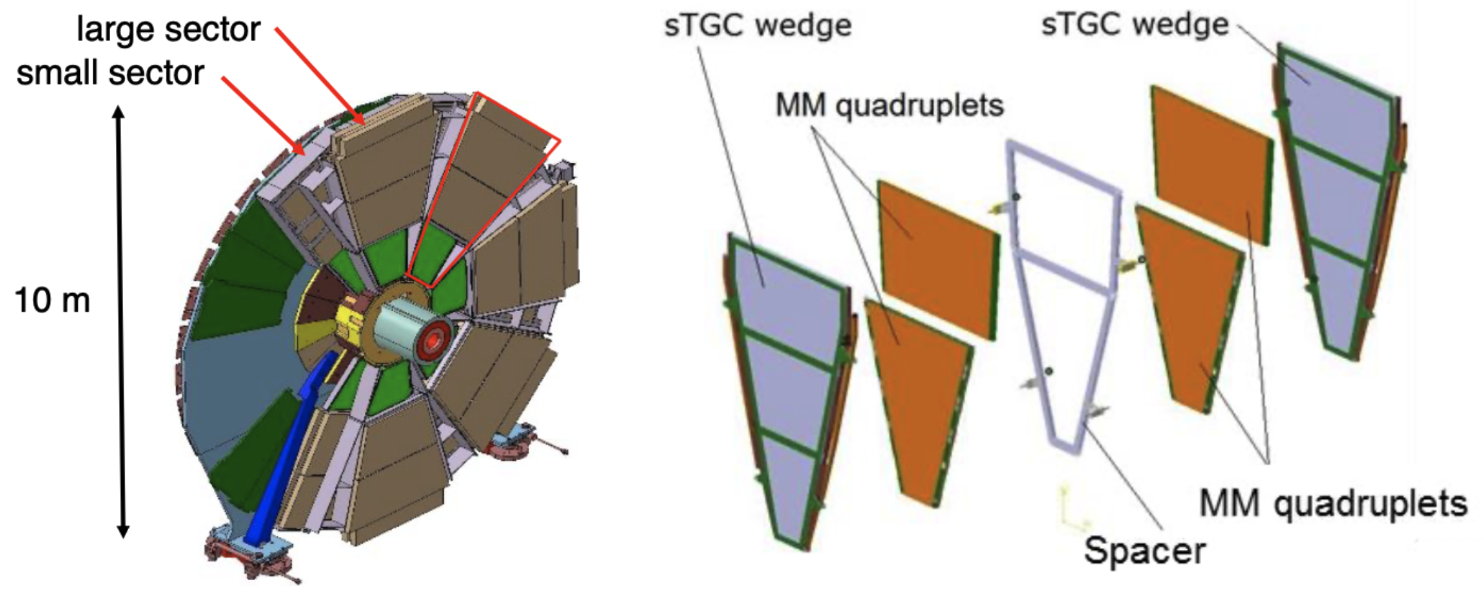
\includegraphics[clip, width=11cm]{fig/2/nsw-structure.png}
  \caption{NSW の構造\cite{article:NSW}。Large Sector と Small Sector の2種類のチェンバーを交互に配置している。sTGC quadruplet の間に、4 層で構成されている MM が 2 つ挟まれており、合計 16 層で構成されている。}
  \label{fig:NSW}
\end{figure}

\subsubsection{small-strip TGC (sTGC)}
small-strip TGC~(sTGC)はTGCと同様の2.8~mmのガスギャップを持つMWPCである。図~\ref{fig:sTGC}に示すようにsTGCはTGCと異なり、ストリップを用いて$\eta$方向の位置座標を、ワイヤーを用いて$\phi$方向の位置座標を測定する。sTGCにはパッドと呼ばれる読み出しカソードがあり、ストリップとパッドでアノードワイヤーを挟む構造になっている。パッドは長方形の電極であり、まずパッドを用いて大まかな位置情報を計算し信号を読み出す領域を限定する。そして、限定された領域のストリップ情報を用いてより精密な位置情報の計算を行うことで高速な飛跡再構成を行う。

\begin{figure}[tb]
  \centering
  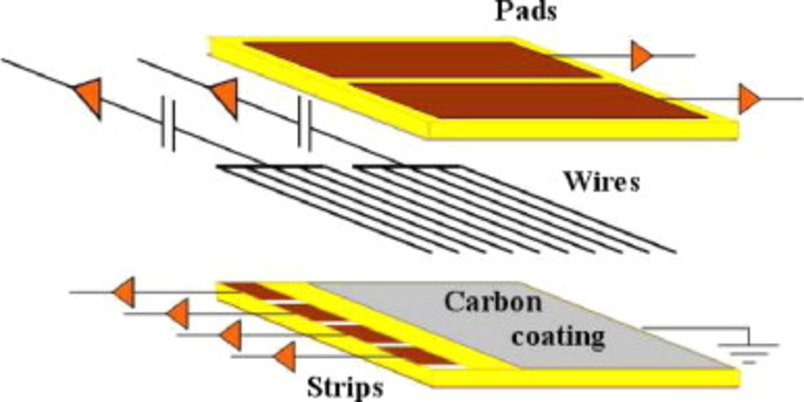
\includegraphics[clip, width=10cm]{fig/2/stgc-structure.pdf}
  \caption{sTGC の断面図\cite{article:sTGC}。 パッド、ストリップを用いて $\eta$ を、ワイヤーを用いて $\phi$ を計算する。}
  \label{fig:sTGC}
\end{figure}

\subsubsection{Micromegas (MM)}
Micromegas~(MM) は、ワイヤーを用いないガス検出器である。図~\ref{fig:MM}にMMの概要図を示す。MMは、厚さ5~mmのドリフト領域と128~$\rm{\mu}$mの増幅領域がメッシュで隔てられている構造である。増幅領域では電子のみでなく陽イオンも生成されるが、MMでは増幅領域の厚さが小さいため、高レート環境でも陽イオンによる影響を抑えることができる。
また、読み出された信号の時間差を用いることで飛跡のz方向の情報を再構成することができる。これにより位置分解能90~$\rm{\mu}$mという高い精度での測定が可能である。

\begin{figure}[tb]
  \centering
  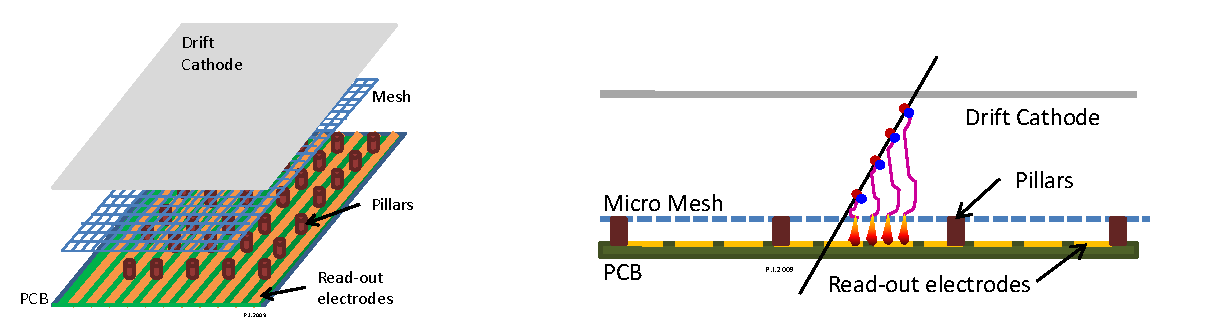
\includegraphics[clip, width=13cm]{fig/2/mm-structure.pdf}
  \caption{MM の概略図\cite{article:sTGC}。メッシュによってドリフト領域と増幅領域に分けられる。ドリフト領域で生成された電子はメッシュを通過し、増幅領域で形成された電場により増幅される。}
  \label{fig:MM}
\end{figure}



\section{ATLAS トリガーシステム}
ATLAS 実験では、LHCを用いて40~MHz での陽子陽子衝突の測定を行っている。しかし、データ記憶容量の制限が存在するためすべての衝突事象を保存することはできず、現在の制約ではトリガーレートを約1~kHzまで削減する必要がある。
そのため、膨大なデータの中から物理として興味のある事象のみを効率よく取得するトリガーシステムを用いて事象選別を行っている。
ATLAS 検出器では大きく分けて 2 段階のトリガーを実装している。1段目にはハードウェアベースの高速処理が可能な初段トリガー~(Level-1 Trigger)、2段目にはソフトウェアベースで精密処理が可能な後段トリガー~(High-Level Trigger) が実装されている。
トリガーシステムの構成を\ref{fig:トリガーの全体像}に示す。

\begin{figure}[tb]
  \centering
  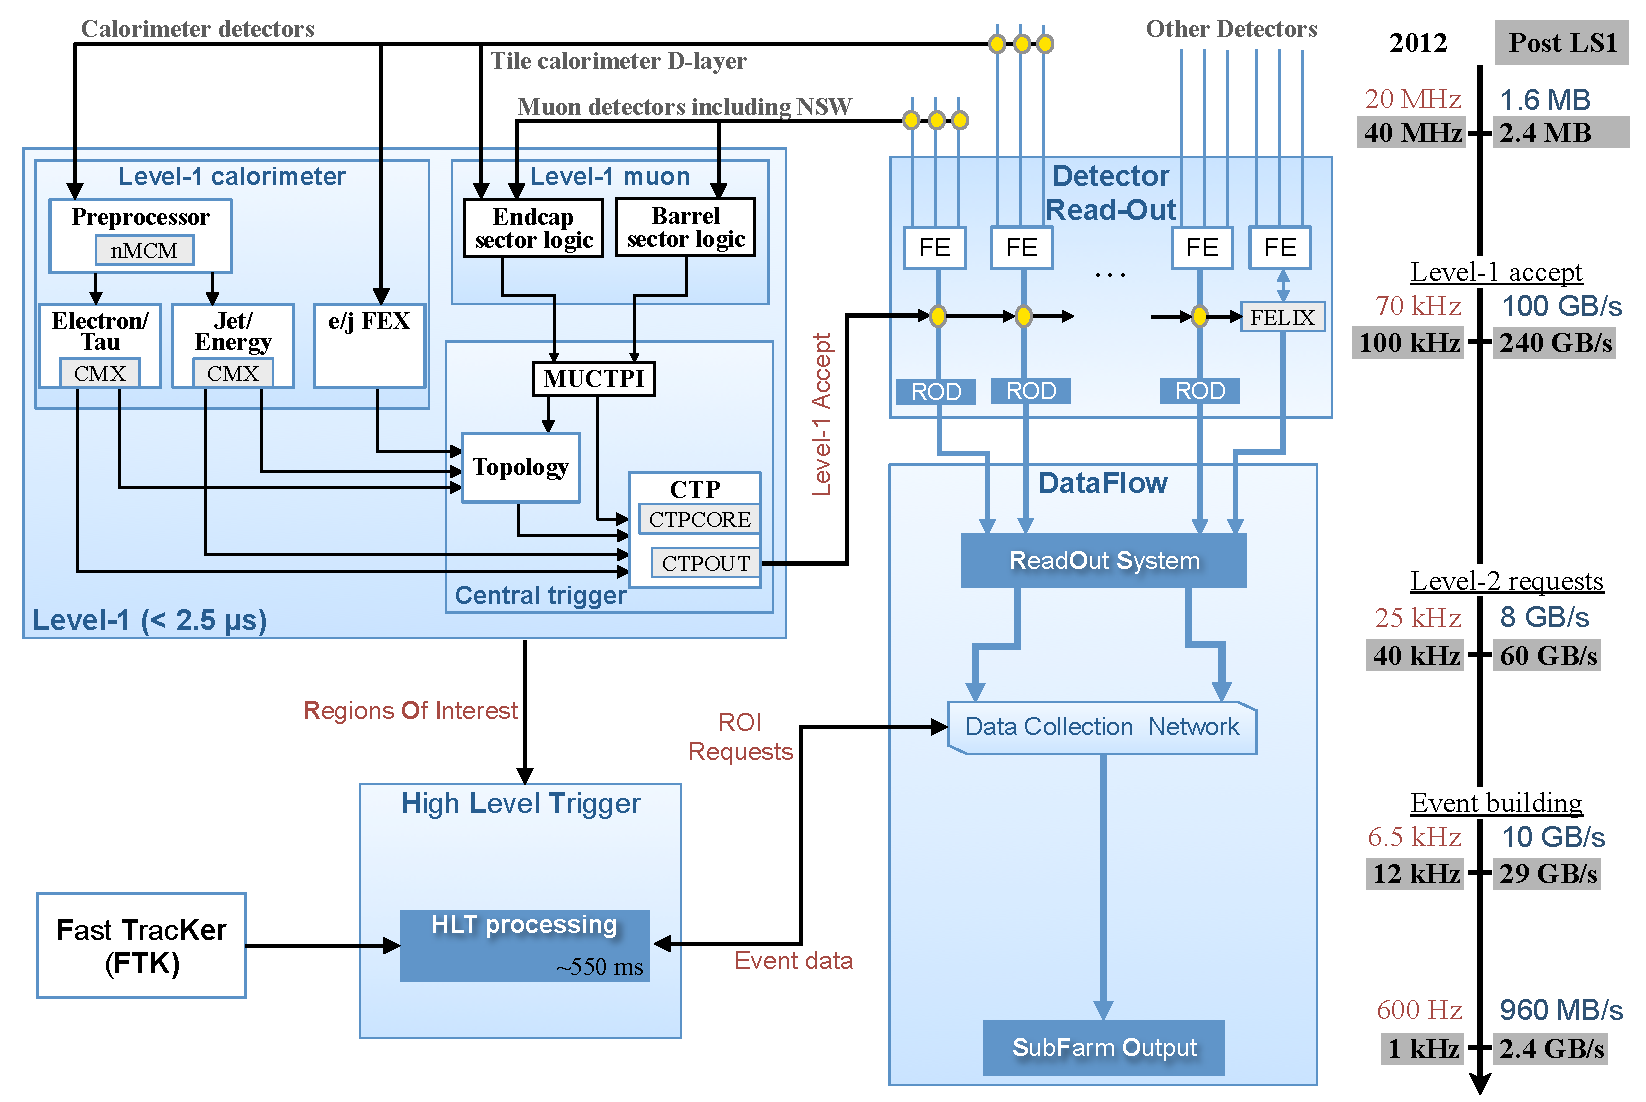
\includegraphics[clip, width=14cm]{fig/3/trigger-nagare2.pdf}
  \caption{Run-3 における ATLAS トリガーシステム及びデータ読み出しの流れ\cite{article:Run3trigger}。トリガーシステムは Level-1 Trigger と High-Level TRigger の 2 段階のトリガーで構成されている。L1 には L1Calo、L1Muon、L1Topo の 3種類が存在する}
  \label{fig:トリガーの全体像}
\end{figure}

\subsubsection{Level-1 Trigger}
初段トリガーであるLevel-1 Trigger~(L1 Triiger)では、ATLAS検出器から送られてくる40~MHzイベントレートの事象を2.5~$\rm{\mu s}$ 以内にトリガー判定を行い、100~kHzまで落とす必要がある。
図\ref{fig:トリガーの全体像}に示すように、L1 Trigger はカロリメータの情報を用いてトリガー判定を行うL1Calo、ミューオン検出器の情報を用いてトリガー判定を行うL1Muonに加え、これらを組み合わせた複合的なトリガーである Central Trigger から構成されている。L1 では、初めにカロリメータとミューオン検出器の情報からそれぞれ単独にトリガー判定を行う。

L1Calo は電磁カロリメータとハドロンカロリメータの情報を統合して、電子/光子と $\tau$ 候補、ジェット候補の判定を行う。

L1Muon はバレル部の RPC とエンドキャップ部の TGC から情報を受け取り、それぞれ独立にトリガー判定を行う。バレル部とエンドキャップ部で独立に判定された L1Muon の情報はMuon-to-CTP interface (MUCTPI) で統合される。

その後、L1Calo と L1Muon からの情報は Central Trigger Processor~(CTP) に送られるのと同時に、TopologyProcessor~(L1Topo) に送られる。L1Topo では L1Muon と L1Calo の情報を組み合わせて、それぞれの情報から複合的なトリガーを発行する。
最後に L1Muon、L1Calo、L1Topo の情報は CTP に集められ、100~kHzに収まるように処理された後に L1Accept~(L1A)としてトリガー発行される。

\subsubsection{High-Level Trigger}
High-Level Trigger (HLT) は Level-1 Trigger より精密なトリガー判定を行う。
HLT では、L1 Trigger で用いられなかった内部飛跡検出器の情報、MDT や CSC などの精密測定用のミューオン検出器の情報、L1Calo のカロリメータの情報などを用いて、飛跡再構成やより高精度な $E_T$、$p_T$ の計算を行う。トリガーレートは HLT を用いて最終的に数 kHz まで削減される。

\subsection{トリガーメニュー}
ATLAS 実験で用いられているトリガーシステムは、限られたレートの中に必要な情報を収めなければならない。初段トリガー、後段トリガーにおけるトリガー要求を合わせたものをトリガーチェインを呼び、トリガーチェインとトリガーレートの配分をまとめたものがトリガーメニューである。
図\ref{fig:muon_trigger_menu.pdf}に Run-3 におけるL1のミューオントリガーメニューを示す。
\begin{figure}[b]
  \centering
  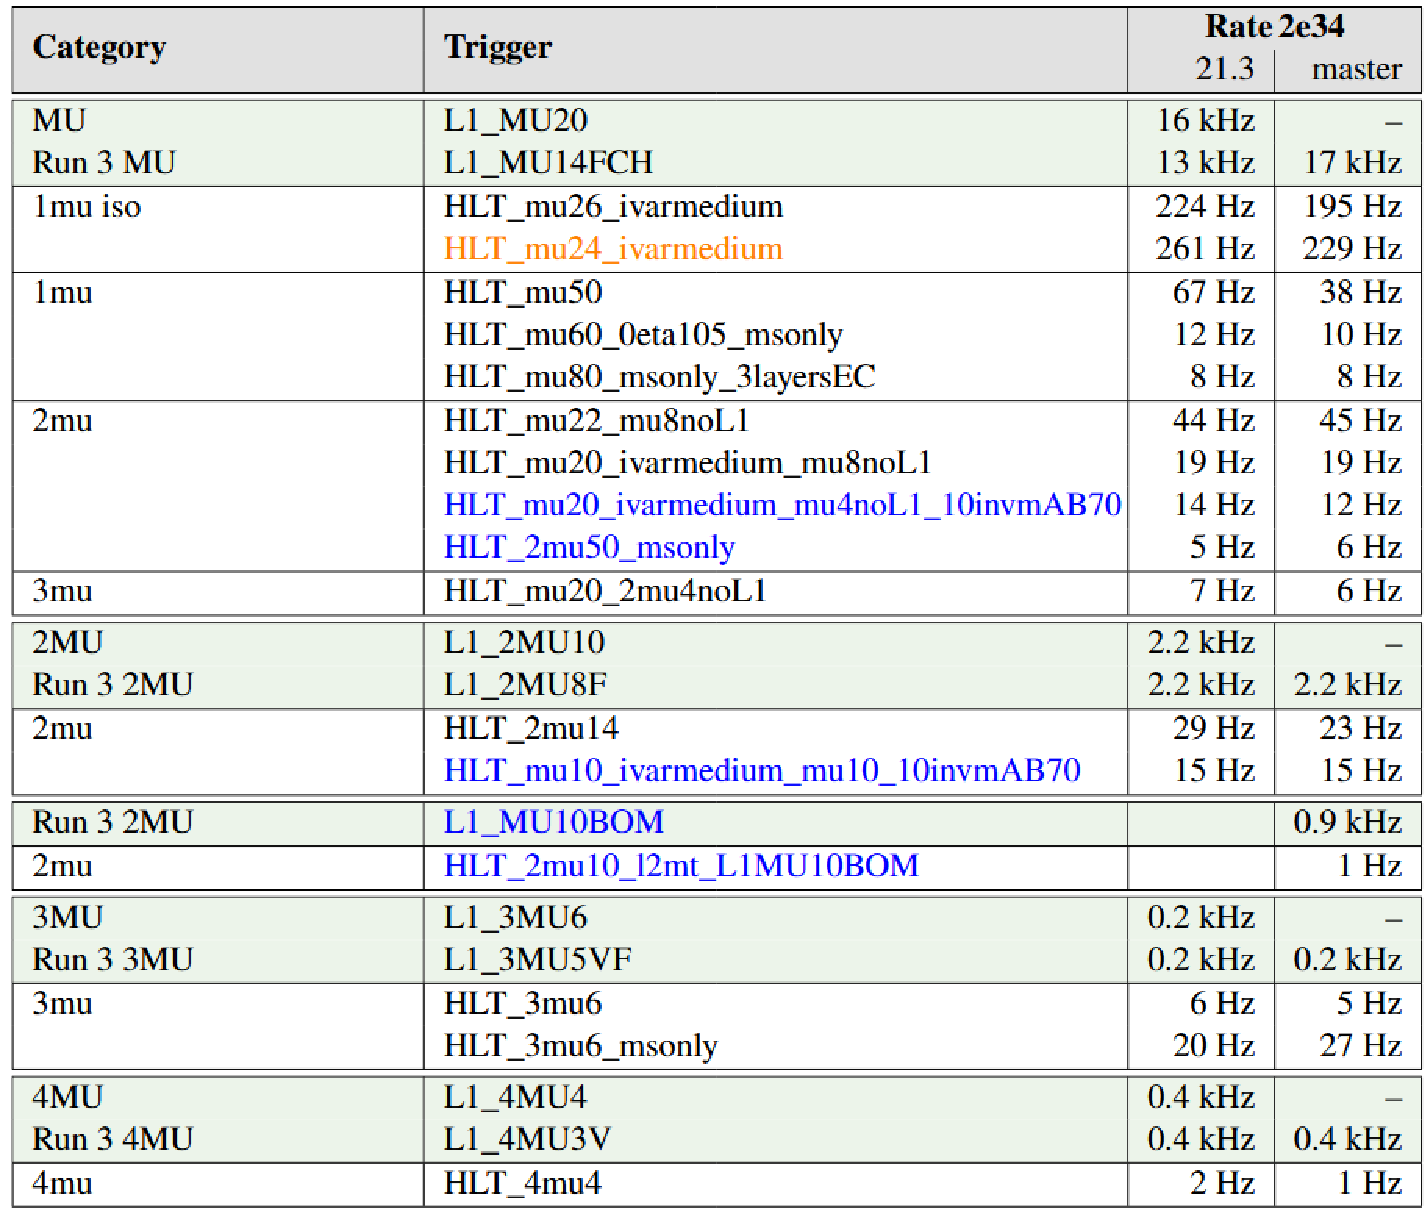
\includegraphics[clip, width=14cm]{fig/2/muon_trigger_menu.pdf}
  \caption{Run-3 におけるプライマリーミューオントリガーのメニュー\cite{article:Run3trigmenu}。}
  \label{fig:muon_trigger_menu.pdf}
\end{figure}

